\PassOptionsToPackage{unicode=true}{hyperref} % options for packages loaded elsewhere
\PassOptionsToPackage{hyphens}{url}
\PassOptionsToPackage{dvipsnames,svgnames*,x11names*}{xcolor}
%
\documentclass[]{book}
\usepackage{lmodern}
\usepackage{amssymb,amsmath}
\usepackage{ifxetex,ifluatex}
\usepackage{fixltx2e} % provides \textsubscript
\ifnum 0\ifxetex 1\fi\ifluatex 1\fi=0 % if pdftex
  \usepackage[T1]{fontenc}
  \usepackage[utf8]{inputenc}
  \usepackage{textcomp} % provides euro and other symbols
\else % if luatex or xelatex
  \usepackage{unicode-math}
  \defaultfontfeatures{Ligatures=TeX,Scale=MatchLowercase}
\fi
% use upquote if available, for straight quotes in verbatim environments
\IfFileExists{upquote.sty}{\usepackage{upquote}}{}
% use microtype if available
\IfFileExists{microtype.sty}{%
\usepackage[]{microtype}
\UseMicrotypeSet[protrusion]{basicmath} % disable protrusion for tt fonts
}{}
\IfFileExists{parskip.sty}{%
\usepackage{parskip}
}{% else
\setlength{\parindent}{0pt}
\setlength{\parskip}{6pt plus 2pt minus 1pt}
}
\usepackage{xcolor}
\usepackage{hyperref}
\hypersetup{
            pdftitle={Einführung in die mathematische Datenanalyse},
            pdfauthor={Jan Heiland},
            colorlinks=true,
            linkcolor=Maroon,
            filecolor=Maroon,
            citecolor=Blue,
            urlcolor=purple,
            breaklinks=true}
\urlstyle{same}  % don't use monospace font for urls
\usepackage{color}
\usepackage{fancyvrb}
\newcommand{\VerbBar}{|}
\newcommand{\VERB}{\Verb[commandchars=\\\{\}]}
\DefineVerbatimEnvironment{Highlighting}{Verbatim}{commandchars=\\\{\}}
% Add ',fontsize=\small' for more characters per line
\usepackage{framed}
\definecolor{shadecolor}{RGB}{248,248,248}
\newenvironment{Shaded}{\begin{snugshade}}{\end{snugshade}}
\newcommand{\AlertTok}[1]{\textcolor[rgb]{0.94,0.16,0.16}{#1}}
\newcommand{\AnnotationTok}[1]{\textcolor[rgb]{0.56,0.35,0.01}{\textbf{\textit{#1}}}}
\newcommand{\AttributeTok}[1]{\textcolor[rgb]{0.77,0.63,0.00}{#1}}
\newcommand{\BaseNTok}[1]{\textcolor[rgb]{0.00,0.00,0.81}{#1}}
\newcommand{\BuiltInTok}[1]{#1}
\newcommand{\CharTok}[1]{\textcolor[rgb]{0.31,0.60,0.02}{#1}}
\newcommand{\CommentTok}[1]{\textcolor[rgb]{0.56,0.35,0.01}{\textit{#1}}}
\newcommand{\CommentVarTok}[1]{\textcolor[rgb]{0.56,0.35,0.01}{\textbf{\textit{#1}}}}
\newcommand{\ConstantTok}[1]{\textcolor[rgb]{0.00,0.00,0.00}{#1}}
\newcommand{\ControlFlowTok}[1]{\textcolor[rgb]{0.13,0.29,0.53}{\textbf{#1}}}
\newcommand{\DataTypeTok}[1]{\textcolor[rgb]{0.13,0.29,0.53}{#1}}
\newcommand{\DecValTok}[1]{\textcolor[rgb]{0.00,0.00,0.81}{#1}}
\newcommand{\DocumentationTok}[1]{\textcolor[rgb]{0.56,0.35,0.01}{\textbf{\textit{#1}}}}
\newcommand{\ErrorTok}[1]{\textcolor[rgb]{0.64,0.00,0.00}{\textbf{#1}}}
\newcommand{\ExtensionTok}[1]{#1}
\newcommand{\FloatTok}[1]{\textcolor[rgb]{0.00,0.00,0.81}{#1}}
\newcommand{\FunctionTok}[1]{\textcolor[rgb]{0.00,0.00,0.00}{#1}}
\newcommand{\ImportTok}[1]{#1}
\newcommand{\InformationTok}[1]{\textcolor[rgb]{0.56,0.35,0.01}{\textbf{\textit{#1}}}}
\newcommand{\KeywordTok}[1]{\textcolor[rgb]{0.13,0.29,0.53}{\textbf{#1}}}
\newcommand{\NormalTok}[1]{#1}
\newcommand{\OperatorTok}[1]{\textcolor[rgb]{0.81,0.36,0.00}{\textbf{#1}}}
\newcommand{\OtherTok}[1]{\textcolor[rgb]{0.56,0.35,0.01}{#1}}
\newcommand{\PreprocessorTok}[1]{\textcolor[rgb]{0.56,0.35,0.01}{\textit{#1}}}
\newcommand{\RegionMarkerTok}[1]{#1}
\newcommand{\SpecialCharTok}[1]{\textcolor[rgb]{0.00,0.00,0.00}{#1}}
\newcommand{\SpecialStringTok}[1]{\textcolor[rgb]{0.31,0.60,0.02}{#1}}
\newcommand{\StringTok}[1]{\textcolor[rgb]{0.31,0.60,0.02}{#1}}
\newcommand{\VariableTok}[1]{\textcolor[rgb]{0.00,0.00,0.00}{#1}}
\newcommand{\VerbatimStringTok}[1]{\textcolor[rgb]{0.31,0.60,0.02}{#1}}
\newcommand{\WarningTok}[1]{\textcolor[rgb]{0.56,0.35,0.01}{\textbf{\textit{#1}}}}
\usepackage{longtable,booktabs}
% Fix footnotes in tables (requires footnote package)
\IfFileExists{footnote.sty}{\usepackage{footnote}\makesavenoteenv{longtable}}{}
\usepackage{graphicx,grffile}
\makeatletter
\def\maxwidth{\ifdim\Gin@nat@width>\linewidth\linewidth\else\Gin@nat@width\fi}
\def\maxheight{\ifdim\Gin@nat@height>\textheight\textheight\else\Gin@nat@height\fi}
\makeatother
% Scale images if necessary, so that they will not overflow the page
% margins by default, and it is still possible to overwrite the defaults
% using explicit options in \includegraphics[width, height, ...]{}
\setkeys{Gin}{width=\maxwidth,height=\maxheight,keepaspectratio}
\setlength{\emergencystretch}{3em}  % prevent overfull lines
\providecommand{\tightlist}{%
  \setlength{\itemsep}{0pt}\setlength{\parskip}{0pt}}
\setcounter{secnumdepth}{5}
% Redefines (sub)paragraphs to behave more like sections
\ifx\paragraph\undefined\else
\let\oldparagraph\paragraph
\renewcommand{\paragraph}[1]{\oldparagraph{#1}\mbox{}}
\fi
\ifx\subparagraph\undefined\else
\let\oldsubparagraph\subparagraph
\renewcommand{\subparagraph}[1]{\oldsubparagraph{#1}\mbox{}}
\fi

% set default figure placement to htbp
\makeatletter
\def\fps@figure{htbp}
\makeatother

\usepackage{xcolor}
\definecolor{jhsc}{HTML}{1f57c7}
\newenvironment {JHSAYS} [0] {\begin{quote}\color{jhsc}} {\end{quote}}

\title{Einführung in die mathematische Datenanalyse}
\author{Jan Heiland}
\providecommand{\institute}[1]{}
\institute{FAU Erlangen-Nürnberg}
\date{FAU Erlangen-Nürnberg -- Sommersemester 2022}

\usepackage{amsthm}
\newtheorem{theorem}{Theorem}[chapter]
\newtheorem{lemma}{Lemma}[chapter]
\newtheorem{corollary}{Corollary}[chapter]
\newtheorem{proposition}{Proposition}[chapter]
\newtheorem{conjecture}{Conjecture}[chapter]
\theoremstyle{definition}
\newtheorem{definition}{Definition}[chapter]
\theoremstyle{definition}
\newtheorem{example}{Example}[chapter]
\theoremstyle{definition}
\newtheorem{exercise}{Exercise}[chapter]
\theoremstyle{definition}
\newtheorem{hypothesis}{Hypothesis}[chapter]
\theoremstyle{remark}
\newtheorem*{remark}{Remark}
\newtheorem*{solution}{Solution}
\begin{document}
\maketitle

{
\hypersetup{linkcolor=}
\setcounter{tocdepth}{1}
\tableofcontents
}
\hypertarget{vorwort}{%
\chapter*{Vorwort}\label{vorwort}}
\addcontentsline{toc}{chapter}{Vorwort}

Das ist ein Aufschrieb.

Korrekturen und Wünsche immer gerne als \emph{issues} oder \emph{pull requests} ans \href{https://github.com/highlando/script-emds}{github-repo}.

\hypertarget{was-ist-data-science}{%
\chapter{Was ist Data Science?}\label{was-ist-data-science}}

Data Science umfasst unter anderem folgende Aufgaben:

\begin{enumerate}
\def\labelenumi{\arabic{enumi}.}
\item
  Strukturieren/Aufbereiten (Umgehen mit falschen, korrumpierten, fehlenden,
  unformatierten Daten)
\item
  Data Exploration (Daten ``verstehen'')
\item
  Data Analysis (quantitative Analysen, Hypothesen aufstellen)
\item
  Data Visualization (Hypothesen graphisch kommunizieren)
\item
  Modelle erzeugen/validieren (Regeln/Muster erkennen, Vorhersagen treffen) -- \emph{das} ist Machine Learning aber es gibt auch viele andere Ansätze.
\item
  Daten Reduktion
\end{enumerate}

\hypertarget{wie-passiert-die-datenanalyse}{%
\section{Wie passiert die Datenanalyse?}\label{wie-passiert-die-datenanalyse}}

Mit mathematischen Methoden aus den Bereichen der

\begin{itemize}
\tightlist
\item
  linearen Algebra (z.B. Matrizen, Basen, lineare Gleichungssysteme)
\item
  Statistik (z.B. Mittelwerte, Korrelationen, Verteilungen)
\item
  Analysis (Grenzwerte, Abschätzungen)
\item
  \ldots{}
\end{itemize}

Dabei hilft Software, z.B.,

\begin{itemize}
\tightlist
\item
  Excel
\item
  \textbf{Python}
\item
  Matlab
\item
  R
\end{itemize}

bei der Berechnung, Automatisierung, Visualisierung.

\begin{quote}
Python ist ein de-facto Standard in Data Science und Machine Learning.
\end{quote}

\hypertarget{was-sind-daten}{%
\section{Was sind Daten?}\label{was-sind-daten}}

Wie sehen Daten aus?

\begin{itemize}
\item
  Numerisch reell, z.B. Temperatur
\item
  Numerisch diskret, z.B. Anzahl
\item
  Ordinal: Element einer festen Menge mit expliziter Ordnung, z.B.
  \{neuwertig, mit Gebrauchsspuren, defekt\}
\item
  Binär: Eine von zwei Möglichkeiten, z.B. Wahr/Falsch oder aktiv/inaktiv
\item
  Kategoriell: Element einer festen Menge ohne klare Ordnung, z.B.
  \{Säugetier, Vogel, Fisch\}
\item
  sonstige strukturierte Daten, z.B. geographische Daten, Graphen
\item
  reiner Text, z.B. Freitext in Restaurantbewertung
\end{itemize}

Außerdem können wir noch allgemeine Eigenschaften (Qualitätsmerkmale) von Daten unterscheiden

\begin{itemize}
\tightlist
\item
  strukturiert
\item
  lückenhaft
\item
  fehlerbehaftet (\emph{verrauscht})
\item
  interpretierbar
\item
  geordnet (oder nicht zu ordnen)
\end{itemize}

\hypertarget{beispiele-01-tabellendaten}{%
\section{Beispiele \{\#01-tabellendaten\}}\label{beispiele-01-tabellendaten}}

\hypertarget{tabellendaten-mietpreise}{%
\subsection{Tabellendaten -- Mietpreise}\label{tabellendaten-mietpreise}}

\begin{figure}
\centering
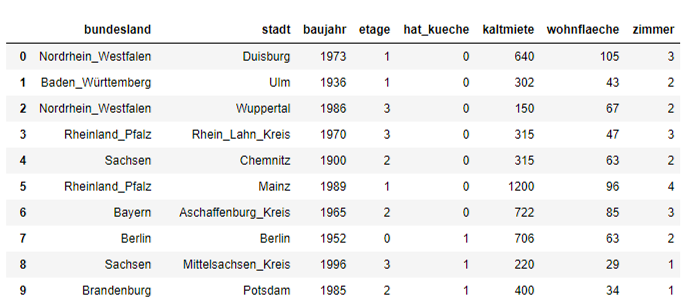
\includegraphics{bilder/dataframe.png}
\caption{Abbildung: Tabelle von Wohnungsangeboten}
\end{figure}

Hier wären die Aufgaben von Data Science:

\begin{itemize}
\tightlist
\item
  Daten ``verstehen'', Zusammenhänge zwischen
  Variablen aufdecken,
\item
  visualisieren.
\item
  Gegebenenfalls fehlende Einträge bei (z.B.) \texttt{kaltmiete} vorhersagen
\end{itemize}

\begin{figure}
\centering
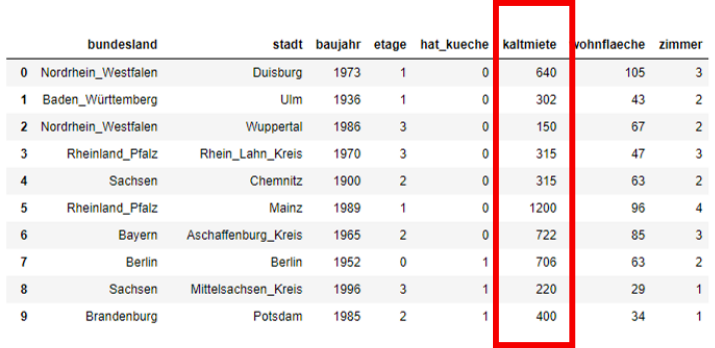
\includegraphics{bilder/dataframe_spalte.png}
\caption{Abbildung: Eine Spalte der Tabelle}
\end{figure}

Datenexploration und -analyse für einzelne Variablen 1/3 Wir betrachten
eine \emph{numerische} Variable in einem rechteckigen Datensatz, also eine
\emph{Spalte} (z.B. \texttt{kaltmiete}). Wir bezeichnen den \(i\)-ten Eintrag in
dieser Spalte mit \(x_i\), wobei \(i=1,\ldots,N\) (\(N\) Anzahl der Zeilen).

Folgende \emph{Schätzer}/\emph{Metriken} können dabei helfen, diese Spalte besser
zu verstehen:

\begin{itemize}
\item
  Mittelwert \(\overline x= \frac1 N\sum_{i=1}^N x_i\)
\item
  gewichteter Mittelwert
  \(\overline x_w = \frac{\sum_{i=1}^N w_i x_i}{\sum_{j=1}^N w_j}\),
  wobei \(w_i\) das Gewicht des \(i\)-ten Eintrages ist (z.B. eine andere
  Variable).
\item
  Varianz: \(s_x^2 = \frac{1}{N-1} \sum_{i=1}^N (x_i-\overline x)^2\)
\item
  Standardabweichung \(s = \sqrt{s_x^2}\).
\item
  Median = \(\frac{315 + 400}{2} = 357.5\).
\end{itemize}

Datenexploration und -analyse für mehrere Variablen Wir betrachten zwei
Spalten \(x = (x_1,\ldots,x_N)\) und \(y = (y_1,\ldots, y_N)\).\\

Das Verteilung von zwei Variablen läßt sich im sogenannte \textbf{Scatter Plot} visualisieren.

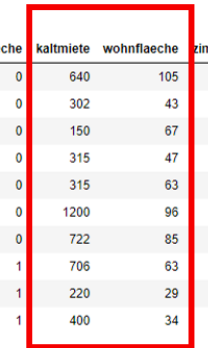
\includegraphics[width=0.27\textwidth,height=\textheight]{bilder/dataframe_spalte3.png}
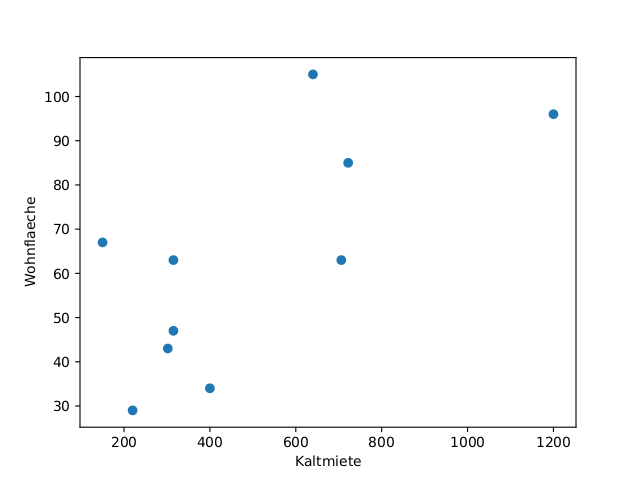
\includegraphics[width=0.7\textwidth,height=\textheight]{bilder/scatterplot.png}

Datenexploration und -analyse für mehrere Variablen Wir betrachten zwei
Spalten \(x = (x_1,\ldots,x_N)\) und \(y = (y_1,\ldots, y_N)\).

\begin{itemize}
\item
  Kovarianz
  \(s_{xy} = \frac{1}{N-1}\sum_{i=1}^N (x_i - \overline x)(y_i - \overline y)\)
\item
  Korrelation \(\rho_{xy} = \frac{s_{xy}}{s_x\cdot s_y} \in [-1,1]\).
\item
  \(\rho \approx 1\): Starke positive Korrelation, wenn \(x\) groß ist,
  ist \(y\) auch groß.
\item
  \(\rho \approx -1\): Starke negative Korrelation, wenn \(x\) groß ist,
  ist \(y\) klein
\item
  \(\rho \approx 0\): Wenig/keine Korrelation.
\end{itemize}

\begin{figure}
\centering
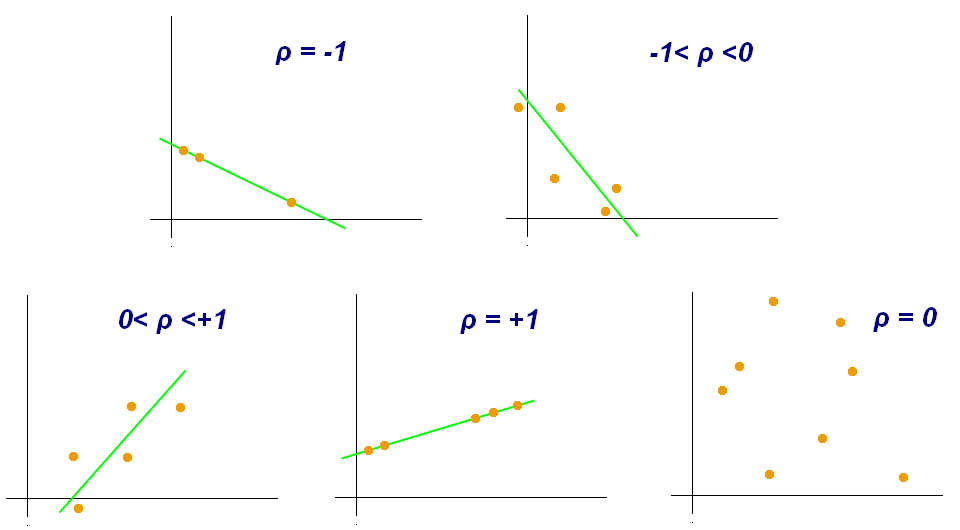
\includegraphics[width=0.65\textwidth,height=\textheight]{bilder/Correlation_coefficient.png}
\caption{Von Kiatdd - Eigenes Werk, CC BY-SA 3.0, \url{https://commons.wikimedia.org/w/index.php?curid=37108966}}
\end{figure}

\hypertarget{covid-19-daten}{%
\subsection{COVID-19 Daten}\label{covid-19-daten}}

Vergleiche die Einführung in \emph{Mathematik für Data Science 1} vom letzten Semester.

\hypertarget{netflix-prize}{%
\subsection{Netflix Prize}\label{netflix-prize}}

Hierbei geht es darum, ob aus bekannten Bewertungen von vielen verschiedenen Benutzern für viele verschiedene Filme abgeleitet werden kann, ob ein bestimmter Nutzer einen bestimmten Film mag (also positiv bewerten würde).

Vergleiche auch \href{https://en.wikipedia.org/wiki/Netflix_Prize}{Wikipedia:Netflix\_Prize}

Das (Trainings-)Daten bestehen über \texttt{480189} Benutzer, die für \texttt{17770} Filme insgesamt \texttt{100480507} Bewertungen als ganze Zahlen zwischen \texttt{1} und \texttt{5} verteilten.

Ziel der Datenanalyse war es, für \texttt{2817131} ``Paare'' von Benutzern und Filmen, die Bewertung vorauszusagen. Neben der schieren Masse an Daten kamen noch Einschränkungen hinzu, die ein Mindestmaß an Qualität der Vorhersage sicherstellen sollten.

Das Problem ließe sich wie folgt darstellen.

\begin{longtable}[]{@{}cccccc@{}}
\toprule
Benutzer \textbackslash{} Film & \texttt{F1} & \texttt{F2} & \texttt{...} & \texttt{Fn} & \texttt{...}\tabularnewline
\midrule
\endhead
\texttt{B1} & -- & 3 & \texttt{...} & 5 & \texttt{...}\tabularnewline
\texttt{B2} & 3 & 4 & \texttt{...} & 2 & \texttt{...}\tabularnewline
\texttt{B3} & 1 & 2 & \texttt{...} & \textbf{?} & \texttt{...}\tabularnewline
\texttt{...} & 3 & 4 & \texttt{...} & -- & \texttt{...}\tabularnewline
\bottomrule
\end{longtable}

Gegeben viele (aber bei weitem nicht alle) Einträge in einer riesigen Tabelle. Können wir aus den Zusammenhängen bestimmte fehlende Einträge (z.B. wie findet Nutzer \texttt{B3} den Film \texttt{Fn}) herleiten?

Die besten Lösungen für dieses Problem basieren durchweg auf \emph{Machine Learning} Ansätzen.

\hypertarget{python}{%
\section{Python}\label{python}}

Die Programmiersprache \texttt{python} wird uns durchs Semester begleiten. Einfach weil sie so wichtig ist für \emph{Data Science} aber auch weil sie (meiner Meinung nach) einfach zu erlernen und zu benutzen ist.

\hypertarget{aufgaben}{%
\section{Aufgaben}\label{aufgaben}}

\hypertarget{python-1}{%
\subsection{Python}\label{python-1}}

Bringen sie ihr \texttt{python} zum Laufen, installieren sie \texttt{numpy}, \texttt{scipy} und \texttt{matplotlib} und führen sie das folgende script aus.

\begin{Shaded}
\begin{Highlighting}[]
\ImportTok{import}\NormalTok{ numpy }\ImportTok{as}\NormalTok{ np}
\ImportTok{import}\NormalTok{ matplotlib.pyplot }\ImportTok{as}\NormalTok{ plt}

\NormalTok{N }\OperatorTok{=} \DecValTok{20}
\NormalTok{xmax }\OperatorTok{=} \DecValTok{2}
\NormalTok{xmin }\OperatorTok{=} \DecValTok{0}

\NormalTok{xdata }\OperatorTok{=}\NormalTok{ np.linspace(xmin, xmax, N)}
\NormalTok{ydata }\OperatorTok{=}\NormalTok{ np.exp(xdata)}

\NormalTok{plt.figure(}\DecValTok{1}\NormalTok{)}
\NormalTok{plt.plot(xdata, ydata, }\StringTok{'.'}\NormalTok{)}

\NormalTok{plt.figure(}\DecValTok{2}\NormalTok{)}
\NormalTok{plt.semilogy(xdata, ydata, }\StringTok{'.'}\NormalTok{)}
\NormalTok{plt.show()}
\end{Highlighting}
\end{Shaded}

\hypertarget{einheitsmatrix}{%
\subsection{Einheitsmatrix}\label{einheitsmatrix}}

Schreiben sie ein script, dass die \texttt{5x5} Einheitsmatrix auf 3 verschiedene Arten erzeugt. (Eine Art könnte die eingebaute \texttt{numpy} Funktion \texttt{eye} sein).

\begin{Shaded}
\begin{Highlighting}[]
\ImportTok{import}\NormalTok{ numpy }\ImportTok{as}\NormalTok{ np}

\NormalTok{idfive }\OperatorTok{=}\NormalTok{ np.eye(}\DecValTok{5}\NormalTok{)}
\BuiltInTok{print}\NormalTok{(idfive)}
\end{Highlighting}
\end{Shaded}

Hinweis: schauen sie sich mal an wie \texttt{numpy}'s \texttt{arrays} funktionieren.

\hypertarget{matrizen-multiplikation-und-potenz}{%
\subsection{Matrizen Multiplikation und Potenz}\label{matrizen-multiplikation-und-potenz}}

Schreiben sie ein script, das die Übungsaufgabe aus der Vorlesung (potenzieren der Matrizen \(M_i\), \(i=1,2,3,4\)) löst. Zum Beispiel mit

\begin{Shaded}
\begin{Highlighting}[]
\ImportTok{import}\NormalTok{ numpy }\ImportTok{as}\NormalTok{ np}
\NormalTok{mone }\OperatorTok{=}\NormalTok{ np.array([[}\FloatTok{0.9}\NormalTok{, }\FloatTok{0.9}\NormalTok{], [}\FloatTok{0.9}\NormalTok{, }\FloatTok{0.9}\NormalTok{]])}

\NormalTok{mone_ptwo }\OperatorTok{=}\NormalTok{ mone }\OperatorTok{@}\NormalTok{ mone}
\BuiltInTok{print}\NormalTok{(mone_ptwo)}

\NormalTok{mone_pfour }\OperatorTok{=}\NormalTok{ mone_ptwo }\OperatorTok{@}\NormalTok{ mone_ptwo}
\BuiltInTok{print}\NormalTok{(mone_pfour)}
\end{Highlighting}
\end{Shaded}

Oder so:

\begin{Shaded}
\begin{Highlighting}[]
\ImportTok{import}\NormalTok{ numpy }\ImportTok{as}\NormalTok{ np}
\NormalTok{mone }\OperatorTok{=}\NormalTok{ np.array([[}\FloatTok{0.9}\NormalTok{, }\FloatTok{0.9}\NormalTok{], [}\FloatTok{0.9}\NormalTok{, }\FloatTok{0.9}\NormalTok{]])}
\NormalTok{mone_p }\OperatorTok{=}\NormalTok{ np.eye(}\DecValTok{2}\NormalTok{)}

\ControlFlowTok{for}\NormalTok{ k }\KeywordTok{in} \BuiltInTok{range}\NormalTok{(}\DecValTok{16}\NormalTok{):}
\NormalTok{    mone_p }\OperatorTok{=}\NormalTok{ mone_p }\OperatorTok{@}\NormalTok{ mone}
    \ControlFlowTok{if}\NormalTok{ k }\OperatorTok{==} \DecValTok{1} \KeywordTok{or}\NormalTok{ k }\OperatorTok{==} \DecValTok{3} \KeywordTok{or}\NormalTok{ k }\OperatorTok{==} \DecValTok{15}\NormalTok{:}
        \BuiltInTok{print}\NormalTok{(}\StringTok{'k='}\NormalTok{, k}\OperatorTok{+}\DecValTok{1}\NormalTok{)}
        \BuiltInTok{print}\NormalTok{(mone_p)}
\end{Highlighting}
\end{Shaded}

Achtung:

\begin{itemize}
\tightlist
\item
  bei Matrizen kann auch \texttt{*} benutzt werden -- das ist aber nicht die richtige Matrizenmultiplikation (sondern die Multiplikation eintragsweise)
\item
  Moegliche Realisierung der Matrizenmultiplikation

  \begin{itemize}
  \tightlist
  \item
    \texttt{np.dot(A,\ B)} -- die klassische Methode
  \item
    \texttt{A.dot(B)} -- das selbe (manchmal besser, wenn \texttt{A} etwas allgemeiner ist (zum Beispiel eine \texttt{scipy.sparse} matrix)
  \item
    \texttt{A\ @\ B} -- convenience Notation
  \end{itemize}
\end{itemize}

\hypertarget{lineare-regression}{%
\chapter{Lineare Regression}\label{lineare-regression}}

Auch bekannt als

\begin{itemize}
\tightlist
\item
  \emph{lineare Ausgleichsrechnung} oder
\item
  \emph{Methode der kleinsten Quadrate}.
\end{itemize}

Ein wesentlicher Aspekt von \emph{Data Science} ist die Analyse oder das
Verstehen von Daten. Allgemein gesagt, es wird versucht, aus den Daten
heraus Aussagen über Trends oder Eigenschaften des Phänomens zu treffen,
mit welchem die Daten im Zusammenhang stehen.

Wir kommen nochmal auf das Beispiel aus der Einführungswoche zurück, werfen eine bereits geschärften Blick darauf und gehen das mit verbesserten mathematischen Methoden an.

Gegeben seien die Fallzahlen aus der CoVID Pandemie 2020 für Bayern für den Oktober 2020.

\hypertarget{tab:covid-cases}{}
\begin{longtable}[]{@{}llllllllllll@{}}
\caption{Anzahl der SARS-CoV-2 Neuinfektionen in Bayern im Oktober 2020.}\tabularnewline
\toprule
Tag & 1 & 2 & 3 & 4 & 5 & 6 & 7 & 8 & 9 & 10 & 11\tabularnewline
\midrule
\endfirsthead
\toprule
Tag & 1 & 2 & 3 & 4 & 5 & 6 & 7 & 8 & 9 & 10 & 11\tabularnewline
\midrule
\endhead
Fälle & 352 & 347 & 308 & 151 & 360 & 498 & 664 & 686 & 740 & 418 & 320\tabularnewline
\bottomrule
\end{longtable}

\begin{longtable}[]{@{}lllllllllll@{}}
\toprule
Tag & 12 & 13 & 14 & 15 & 16 & 17 & 18 & 19 & 20 & 21\tabularnewline
\midrule
\endhead
Fälle & 681 & 691 & 1154 & 1284 & 127 & 984 & 573 & 1078 & 1462 & 2239\tabularnewline
\bottomrule
\end{longtable}

\begin{longtable}[]{@{}lllllllllll@{}}
\toprule
Tag & 22 & 23 & 24 & 25 & 26 & 27 & 28 & 29 & 30 & 31\tabularnewline
\midrule
\endhead
Fälle & 2236 & 2119 & 1663 & 1413 & 2283 & 2717 & 3113 & 2972 & 3136 & 2615\tabularnewline
\bottomrule
\end{longtable}

\begin{figure}
\hypertarget{fig:cases}{%
\centering
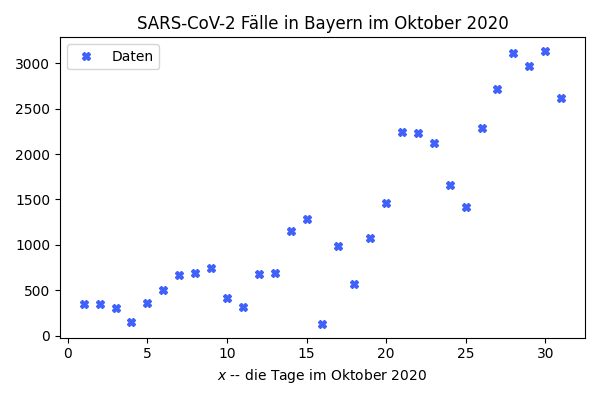
\includegraphics{bilder/02-cases.png}
\caption{Fallzahlen von Sars-CoV-2 in Bayern im Oktober
2020}\label{fig:cases}
}
\end{figure}

Wieder stellen wir uns die Frage ob wir \textbf{in den Daten einen funktionalen
Zusammenhang} feststellen können. Also ob wir die Datenpaare

\begin{quote}
(Tag \(x\), Infektionen am Tag \(x\))
\end{quote}

die wir als

\begin{quote}
(\(x_i\), \(y_i\))
\end{quote}

über eine Funktion \(f\) und die Paare

\begin{quote}
(\(x\), \(f(x)\))
\end{quote}

beschreiben (im Sinne von gut darstellen oder approximieren) können.

\hypertarget{rauschen-und-fitting}{%
\section{Rauschen und Fitting}\label{rauschen-und-fitting}}

Beim obigen Beispiel (und ganz generell bei Daten) ist davon auszugehen, dass die Daten \textbf{verrauscht} sind, also einem Trend folgen oder in einem funktionalen Zusammenhang stehen aber zufällige Abweichungen oder Fehler enthalten.

Unter diesem Gesichtspunkt ist eine Funktion, die

\begin{quote}
\(f(x_i)=y_i\)
\end{quote}

erzwingt nicht zielführend. (Wir wollen Trends und größere Zusammenhänge erkennen und nicht kleine Fehler nachzeichnen.) Das zu strenge Anpassen an möglicherweise verrauschte Daten wird \textbf{overfitting} genannt.

Vielmehr werden wir nach einer Funktion \(f\) suchen, die die Daten näherungsweise nachstellt:

\begin{quote}
\(f(x_i)\approx y_i\)
\end{quote}

Hierbei passen jetzt allerdings auch Funktionen, die vielleicht einfach zu handhaben sind aber die Daten kaum noch repräsentieren. Jan spricht von \textbf{underfitting}.

Eine gute Approximation besteht im Kompromiss von \emph{nah an den Daten} aber mit wenig \emph{overfitting}.

\hypertarget{ansuxe4tze-fuxfcr-lineare-regression}{%
\section{Ansätze für lineare Regression}\label{ansuxe4tze-fuxfcr-lineare-regression}}

Um eine solche Funktion \(f\) zu finden, trifft Jan als erstes ein paar
Modellannahmen. Modellannahmen legen fest, wie das \(f\) im Allgemeinen
aussehen soll und versuchen dabei

\begin{enumerate}
\def\labelenumi{\arabic{enumi}.}
\item
  die Bestimmung von \(f\) zu ermöglichen
\item
  zu garantieren, dass \(f\) auch die gewollten Aussagen liefert
\item
  und sicherzustellen, dass \(f\) zum Problem passt.
\end{enumerate}

Jan bemerke, dass die ersten beiden Annahmen im Spannungsverhältnis zur
dritten stehen.

\textbf{Lineare Regression} besteht darin, dass die Funktion als Linearkombination

\begin{equation*}
f_w(x) = \sum_{j=1}^n w_j b_j(x)
\end{equation*}

von Basisfunktionen geschrieben wird und dann die \emph{Koeffizienten} \(w_i\) so bestimmt werden, dass \(f\) die Daten bestmöglich annähert.

\begin{quote}
Jan bemerke, dass \emph{bestmöglich} wieder \emph{overfitting} bedeuten kann aber auch, bei schlechter Wahl der Basis, wenig aussagekräftig sein kann. Der gute Kompromiss liegt also jetzt in der Wahl der passenden Basisfunktionen und deren Anzahl. (Mehr Basisfunktionen bedeutet möglicherweise bessere Approximation aber auch die Gefahr von \emph{overfitting}.)
\end{quote}

Typische Wahlen für die Basis \(\{b_1, b_2, \dotsc, b_n\}\) sind

\begin{itemize}
\tightlist
\item
  Polynome: \(\{1, x, x^2, \dotsc, x^{n-1}\}\) -- für \(n=2\) ist der Ansatz \emph{eine Gerade}
\item
  Trigonometrische Funktionen: \(\{1, \cos(x), \sin(x), \cos(2x), \sin(2x), \dotsc\}\)
\item
  Splines -- Polynome, die abschnittsweise definiert werden
\item
  Wavelets -- Verallgemeinerungen von trigonometrischen Funktionen
\end{itemize}

\hypertarget{fehlerfunktional-und-minimierung}{%
\section{Fehlerfunktional und Minimierung}\label{fehlerfunktional-und-minimierung}}

Wir setzen nun also an
\begin{equation*}
f_w(x) = \sum_{j=1}^nw_j b_j (x)
\end{equation*}
und wollen damit \(y_i \approx f_w(x_i)\) \emph{bestmöglich} erreichen (indem wir die Koeffizienten \((w_1, \dotsc, w_n)\) \emph{optimal} wählen. Bestmöglich und optimal spezifizieren wir über den Mittelwert der quadratischen Abweichungen in der Approximation über alle Datenpunkte
\begin{equation*}
\frac{1}{N}\sum_{i=1}^N (y_i - f_w(x_i))^2
\end{equation*}

Ein paar Bemerkungen

\begin{itemize}
\tightlist
\item
  jetzt müssen wir die \(w_i\)'s bestimmen so dass dieser Fehlerterm minimal wird
\item
  das optimale \(w\) ist unabhängig von einer Skalierung des Fehlerterms
\item
  des wegen schreiben wir gerne einfach \(\frac 12 \sum_{i=1}^N (y_i - f_w(x_i))^2\) als das Zielfunktional, das es zu minimieren gilt.
\end{itemize}

Wie finden wir jetzt die \(w_i\)'s? Zunächst gilt, dass
\begin{equation*}
f_w(x_i) = \sum_{i=j}^n w_j b_j(x_i) = 
\begin{bmatrix}
b_1(x_i) & b_2(x_i) & \dots & b_n(x_i)
\end{bmatrix}
\begin{bmatrix}
w_1 \\ w_2 \\ \vdots \\ w_n
\end{bmatrix}
\end{equation*}

und wenn wir alle \(f_w(x_i)\), \(i=1,\dotsc,N\) übereinander in einen Vektor schreiben, dass

\begin{equation*}
f_w(\mathbf x) := 
\begin{bmatrix}
f_w(x_1) \\ \vdots \\ f_w(x_N)
\end{bmatrix}
=
\begin{bmatrix}
b_1(x_1) & \dots & b_n(x_1) \\
\vdots & \ddots & \vdots \\
b_1(x_N) & \dots & b_n(x_N)
\end{bmatrix}
\begin{bmatrix}
w_1 \\ \vdots \\ w_n
\end{bmatrix}
=: \Phi(\mathbf x) w
\end{equation*}

Damit, mit \(\mathbf y\) als den Vektor aller \(y_i\)'s, und mit der Definition der Vektornorm, können wir unser Minimierungsproblem schreiben als
\begin{equation*}
\frac 12  \sum_{i=1}^N (y_i - f_w(x_i))^2 = \frac 12 \| \mathbf y - \Phi (\mathbf x) w\|^2 \to \min.
\end{equation*}

Wir bemerken, dass

\begin{itemize}
\tightlist
\item
  das Fehlerfunktional immer größer und bestenfalls gleich 0 ist
\item
  falls das lineare Gleichungssystem \(\Phi (\mathbf x)w = \mathbf y\) eine Lösung \(w\) hat, ist das auch eine Lösung unserer Minimierung
\item
  im typischen Falle aber ist allerdings \(N\gg n\) und das System überbestimmt (\(n=N\) würde ein overfitting bedeuten\ldots{}) sodass wir keine Lösung des linearen Gleichungssystems erwarten können.
\item
  Das Minimierungsproblems selbst hat allerdings immer eine Lösung.
\end{itemize}

\hypertarget{berechnung-der-bestluxf6sung}{%
\section{Berechnung der Bestlösung}\label{berechnung-der-bestluxf6sung}}

Wir suchen also ein Minimum der Funktion (mit \(\Phi\), \(\mathbf x\), \(\mathbf y\) gegeben)
\begin{equation*}
\begin{split}
w \mapsto \frac 12 \|\mathbf y - \Phi(\mathbf x)w \|^2 &= \frac 12 (\mathbf y - \Phi(\mathbf x)w)^T(\mathbf y - \Phi(\mathbf x)w)  \\ 
&= \frac 12 [\mathbf y^T\mathbf y - \mathbf y^T \Phi(\mathbf x)w - w^T \Phi(\mathbf x)^T\mathbf y  + w^T \Phi(\mathbf x)^T\Phi(\mathbf x)w] \\
&= \frac 12 [\mathbf y^T\mathbf y -2 w^T \Phi(\mathbf x)^T\mathbf y  + w^T \Phi(\mathbf x)^T\Phi(\mathbf x)w] 
\end{split}
\end{equation*}
wobei wir die Definition der Norm \(\|v\|^2 = v^Tv\) und die Eigenschaft, dass für die skalare Größe \(w^T \Phi(\mathbf x)^T\mathbf y = [w^T \Phi(\mathbf x)^T\mathbf y]^T = \mathbf y^T \Phi(\mathbf x)w\) gilt, ausgenutzt haben.

Wären \(w\) und \(\mathbf y\) keine Vektoren sondern einfach reelle Zahlen, wäre das hier eine Parabelgleichung \(aw^2 + bw + c\) mit \(a>0\), die immer eine Minimalstelle hat.

Tatsächlich gilt hier alles ganz analog. Insbesondere ist \(\Phi(\mathbf x)^T\Phi(\mathbf x)\) in der Regel ``größer 0'' (was heißt das wohl bei quadratischen Matrizen?). Und mittels ``Nullsetzen'' der ersten Ableitung können wir das Minimum bestimmen. In diesem Fall ist die erste Ableitung (nach \(w\))
\begin{equation*}
\nabla_w (\frac 12 \|\mathbf y - \Phi(\mathbf x) \|^2) = \Phi(\mathbf x)^T\Phi(\mathbf x)w - \Phi(\mathbf x)^T\mathbf y,
\end{equation*}
(den \emph{Gradienten} \(\nabla_w\) als Ableitung von Funktionen mit mehreren Veränderlichen werden wir noch genauer behandeln)
was uns als Lösung, die Lösung des linearen Gleichungssystems
\begin{equation*}
\Phi(\mathbf x)^T\Phi(\mathbf x)w = \Phi(\mathbf x)^T\mathbf y
\end{equation*}
definiert.

Letzte Frage: Wann hat dieses Gleichungssystems eine eindeutige Lösung? Mit \(N>n\) (also \(\Phi(\mathbf x)\) hat mehr Zeilen als Spalten) gelten die Äquivalenzen:

\begin{itemize}
\tightlist
\item
  \(\Phi(\mathbf x)^T\Phi(\mathbf x)w = \Phi(\mathbf x)^T\mathbf y\) hat eine eindeutige Lösung
\item
  die Matrix \(\Phi(\mathbf x)^T\Phi(\mathbf x)\) ist regulär
\item
  die Spalten von \(\Phi(\mathbf x)\) sind linear unabhängig
\item
  die Vektoren \(b_i(\mathbf x)\) sind linear unabhängig.
\end{itemize}

Praktischerweise tritt genau diese Situation im Allgemeinen ein.

\begin{itemize}
\tightlist
\item
  \(N>n\) (mehr Datenpunkte als Parameter)
\item
  \(b_i\)'s werden als \emph{linear unabhängig} (im Sinne ihres Funktionenraums) gewählt, was die lineare unabhängigket der \(b_i(\mathbf x)\) impliziert.
\end{itemize}

\hypertarget{beispiel}{%
\section{Beispiel}\label{beispiel}}

Unsere Covid-Zahlen ``mit einer Geraden angenähert'':

\begin{itemize}
\tightlist
\item
  \(f_w(x) = w_1 + w_2 x\) -- das heißt \(n=2\) und Basisfunktionen \(b_1(x)\equiv 1\) und \(b_2(x) = x\)
\item
  \(\mathbf x = (1,2,3, \dots, 31)\) -- die Tage im Februar, das heißt \(N=31\)
\item
  \(\mathbf y = (352, 347, \dots, 2615)\) -- die Fallzahlen
\end{itemize}

Wir bekommen

\begin{equation*}
\Phi(\mathbf x) = 
\begin{bmatrix}
1 & 1 \\ 1 & 2 \\ 1 & 3 \\ \vdots & \vdots \\ 1 & 31
\end{bmatrix}
\end{equation*}
(die Spalten sind linear unabhängig) und müssen ``nur'' das 2x2 System
\[
\begin{bmatrix}
1 & 1 & 1 & \dots & 1 \\ 1 & 2 & 3 & \dots & 31
\end{bmatrix}
\begin{bmatrix}
1 & 1 \\ 1 & 2 \\ 1 & 3 \\ \vdots \\ 1 & 31
\end{bmatrix}
\begin{bmatrix}
w_1 \\ w_2
\end{bmatrix}
=
\begin{bmatrix}
1 & 1 & 1 & \dots & 1 \\ 1 & 2 & 3 & \dots & 31
\end{bmatrix} 
\begin{bmatrix}
352 \\  347 \\ 308 \\ \vdots \\ 2615
\end{bmatrix} 
\]
lösen um die Approximation \(f_w\) zu bestimmen.

Und noch als letzte Bemerkung. Egal wie die Basisfunktionen \(b_i\) gewählt werden, die Parameterabhängigkeit von \(w\) ist immer linear. Deswegen der Name \textbf{lineare Ausgleichsrechnung}.

\hypertarget{matrix-zerlegungen}{%
\chapter{Matrix-Zerlegungen}\label{matrix-zerlegungen}}

Die Lösung \(w\) des Problems der \emph{linearen Ausgleichsrechnung} war entweder als Lösung eines Optimierungsproblems
\begin{equation*}
\min_{w} \| Aw - y \|^2
\end{equation*}
oder als Lösung des linearen Gleichungssystems
\begin{equation*}
A^TAw=y
\end{equation*}
gegeben. Hierbei steht nun \(A\in \mathbb R^{N\times n}\) für die Matrix \(\Phi(\mathbf x)\) der Daten und Basisfunktionen. Wir hatten uns überlegt, dass in den meisten Fällen

\begin{itemize}
\tightlist
\item
  die Matrix mehr Zeilen als Spalten hat (\(N>n\)) und
\item
  die Spalten linear unabhängig sind.
\end{itemize}

\hypertarget{qr-zerlegung}{%
\section{QR Zerlegung}\label{qr-zerlegung}}

Wir betrachten nochmal das Optimierungsproblem \(\min_{w} \| Aw - y \|^2\). Gäbe es eine Lösung des Systems \(Aw=y\), wäre das sofort eine Lösung des Optimierungsproblems. Da \(A\) aber mehr Zeilen als Spalten hat, ist das System \(Aw=y\) überbestimmt und eine Lösung in der Regel nicht gegeben.

Die Überlegung ist nun, die Gleichung \(Aw=y\) \emph{so gut wie möglich} zu erfüllen, indem wir die relevanten Gleichungen indentifizieren und wenigstens diese lösen. Ein systematischer (und wie wir später sehen werden auch zum Optimierungsproblem passender) Zugang bietet die QR Zerlegung.

\begin{theorem}[QR Zerlegung]
\protect\hypertarget{thm:qr}{}\label{thm:qr}Sei \(A\in \mathbb R^{m\times n}\), \(m>n\). Dann existiert eine orthonormale Matrix \(Q\in \mathbb R^{m\times m}\) und eine obere Dreiecksmatrix \(\hat R\in \mathbb R^{n\times n}\) derart dass
\begin{equation*}
A = QR =: Q 
\begin{bmatrix}
\hat R \\ 0
\end{bmatrix}.
\end{equation*}
Hat \(A\) vollen (Spalten)Rang, dann ist \(\hat R\) invertierbar.
\end{theorem}

Hier heißt \emph{orthonormale Matrix} \(Q\), dass die Spalten von \(Q\) paarweise orthogonal sind. Insbesondere gilt
\begin{equation*}
Q^T Q = I.
\end{equation*}

Für unser zu lösendes Problem ergibt sich dadurch die Umformung
\begin{equation*}
Aw = y \quad \Leftrightarrow \quad QRw=y \quad \Leftrightarrow \quad Q^TQRw=Q^T y 
 \quad \Leftrightarrow \quad  Rw = Q^Ty
\end{equation*}
oder auch
\begin{equation*}
\begin{bmatrix}
\hat R \\ 0
\end{bmatrix}w 
=
Q^Ty
=
\begin{bmatrix}
Q_1^T \\ Q_2^T
\end{bmatrix}
y
\end{equation*}
(wobei wir die \(Q_1\in \mathbb R^{m\times n}\) die Matrix der ersten \(n\) Spalten von \(Q\) ist)
und als \emph{Kompromiss} der Vorschlag, das Teilsystem
\begin{equation*}
\hat R w = Q_1^Ty
\end{equation*}
nach \(w\) zu lösen und in Kauf zu nehmen, dass der Rest, nämlich das \(Q_2^Ty\), nicht notwendigerweise gleich null ist.

Wir halten zunächst mal fest, dass

\begin{itemize}
\tightlist
\item
  Obwohl \(Q\) eine reguläre Matrix ist, bedarf der Übergang von \(Aw=y\) zu \(Q^TAw=Q^Ty\) einer genaueren Analyse.
\item
  Wir bemerken, dass für eine hypothetische komplette Lösung \(Aw-y\), diese Transformation keine Rolle spielt.
\item
  Für die Kompromisslösung jedoch schon, weil beispielsweise verschiedene Konstruktionen eines invertierbaren Teils, verschiedene Residuen bedeuten und somit Optimalität im Sinne von \(\min_w \|Aw-y\|^2\) nicht garantiert ist.
\end{itemize}

Allerdings, wie Sie als Übungsaufgabe nachweisen werden, löst dieser Ansatz tatsächlich das Optimierungsproblem.

\hypertarget{singuluxe4rwertzerlegung}{%
\section{Singulärwertzerlegung}\label{singuluxe4rwertzerlegung}}

Eine weitere Matrix Zerlegung, die eng mit der Lösung von Optimierungsproblemen oder überbestimmten Gleichungssystemen zusammenhängt ist die \emph{Singulärwertzerlegung} (SVD -- von english: \emph{Singular Value Decomposition}).

\begin{theorem}[Singulärwertzerlegung]
\protect\hypertarget{thm:svd}{}\label{thm:svd}Sei \(A\in \mathbb C^{m\times n}\), \(m\geq n\). Dann existieren orthogonale Matrizen \(U \in \mathbb C^{m\times m}\) und \(V\in \mathbb C^{n\times n}\) und eine Matrix \(\Sigma \in \mathbb R^{m\times n}\) der Form
\begin{equation*}
\Sigma = 
\begin{bmatrix}
\sigma_1 & 0 & \dots & 0\\
0 & \sigma_2 &\ddots & \vdots\\
0 & \ddots & \ddots &0\\
  0 & \dots&0 & \sigma_n \\
  0 & 0 & \dots & 0 \\
  \vdots & \ddots &  & \vdots\\
  0 & 0 & \dots & 0
\end{bmatrix}
\end{equation*}
mit reellen sogenannten \emph{Singulärwerten}
\begin{equation*}
\sigma_1 \geq \sigma_2 \geq \dots \geq \sigma_n \geq 0
\end{equation*}
sodass gilt
\begin{equation*}
A = U \Sigma V^*
\end{equation*}
wobei gilt \(V^* = \overline{V^T}\) (transponiert und komplex konjugiert).
\end{theorem}

Ein paar Bemerkungen.

\begin{itemize}
\tightlist
\item
  Ist \(A\) reell, können auch \(U\) und \(V\) reell gewählt werden.
\item
  Die Annahme \(m \geq n\) war nur nötig um für die Matrix \(\Sigma\) keine Fallunterscheidung zu machen. (Für \(m\leq n\) ``steht der Nullblock rechts von den Singulärwerten''). Insbesondere gilt \(A^* = V\Sigma U^*\) ist eine SVD von \(A^*\).
\item
  Eine Illustration der Zerlegung ist in Abbildung \ref{SVD} zu sehen.
\end{itemize}

Wir machen einige Überlegungen im Hinblick auf große Matrizen. Sei dazu \(m>n\), \(A\in \mathbb C^{m\times n}\) und \(A=U\Sigma V^*\) eine SVD wie in Theorem @ref\{thm:SVD\}. Sei nun
\begin{equation*}
U = \begin{bmatrix}
U_1 & U_2
\end{bmatrix}
% = \begin{bmatrix} V_1^* & V_2^*
\end{equation*}
partitioniert sodass \(U_1\) die ersten \(n\) Spalten von \(U\) enthält.

Dann gilt (nach der Matrix-Multiplikations Regel \emph{Zeile mal Spalte} die Teile \(U_2\) und \(V_2\) immer mit dem Nullblock in \(\Sigma\) multipliziert werden) dass
\begin{equation*}
A = U\Sigma V = 
\begin{bmatrix}
U_1 & U_2
\end{bmatrix}
\begin{bmatrix}
\hat \Sigma \\ 0
\end{bmatrix}
V^*
% \begin{bmatrix} V_1^* \\ V_2^* \end{bmatrix}
=
U_1 
\hat \Sigma
V^*
% \begin{bmatrix} V_1^* \\ V_2^* \end{bmatrix}
\end{equation*}
Es genügt also nur die ersten \(m\) Spalten von \(U\) zu berechnen. Das ist die sogenannte \textbf{slim SVD}.

Hat, darüberhinaus, die Matrix \(A\) keinen vollen Rang, also \(\operatorname{Rg}(A) = r < n\), dann:

\begin{itemize}
\tightlist
\item
  ist \(\sigma_i=0\), für alle \(i=r+1, \dotsc, n\), (wir erinnern uns, dass die Singulärwerte nach Größe sortiert sind)
\item
  die Matrix \(\hat \Sigma\) hat \(n-r\) Nullzeilen
\item
  für die Zerlegung sind nur die ersten \(r\) Spalten von \(U\) und \(V\) relevant -- die sogenannte \textbf{Kompakte SVD}.
\end{itemize}

In der Datenapproximation ist außerdem die \textbf{truncated SVD} von Interesse. Dazu sei \(\hat r<r\) ein beliebig gewählter Index. Dann werden alle Singulärwerte, \(\sigma_i=0\), für alle \(i=\hat r+1, \dotsc, n\), abgeschnitten -- das heißt null gesetzt und die entsprechende \emph{kompakte SVD} berechnet.

Hier gilt nun nicht mehr die Gleichheit in der Zerlegung. Vielmehr gilt
\begin{equation*}
A \approx A_{\hat r}
\end{equation*}
wobei \(A_{\hat r}\) aus der \emph{truncated SVD} von \(A\) erzeugt wurde. Allerdings ist diese Approximation von \(A\) durch optimal in dem Sinne, dass es keine Matrix vom Rang \(\hat r \geq r=\operatorname{Rg}(A)\) gibt, die \(A\) (in der \emph{induzierten} euklidischen Norm\footnote{Auf Matrixnormen kommen wir noch in der Vorlesung zu sprechen.}) besser approximiert. Es gilt
\begin{equation*}
\min_{B\in \mathbb C^{m\times n}, \operatorname{Rg}(B)=\hat r} \|A-B\|_2 = \|A-A_{\hat r}\|_2 = \sigma_{\hat r + 1};
\end{equation*}
vgl. Bollhoefer/Mehrmann Satz 14.15.

Zum Abschluss noch der Zusammenhang zum Optimierungsproblem. Ist \(A=U\Sigma V^*\) ``SV-zerlegt'', dann gilt
\begin{equation*}
A^*Aw = V\Sigma^*U^*U\Sigma V^*w = V\hat \Sigma^2 V^* 
\end{equation*}
und damit
\begin{equation*}
A^*Aw = A^*y \quad \Leftrightarrow \quad V\hat \Sigma^2 V^*  = V\Sigma^*U^*y \quad \Leftrightarrow \quad w = V(\Sigma^+)^*U^*y
\end{equation*}
wobei
\begin{equation*}
\Sigma^+ = \begin{bmatrix}
\hat \Sigma^{-1} \\ 0_{m-n \times n}
\end{bmatrix}
\end{equation*}
aus \(\Sigma \hat \Sigma^{-1}\hat \Sigma^{-1}\) herrührt.

\textbf{Bemerkung}: \(\Sigma^+\) kann auch definiert werden, wenn \(\hat \Sigma\) nicht invertierbar ist (weil manche Diagonaleinträge null sind). Dann wird \(\hat \Sigma^+\) betrachtet, bei welcher nur die \(\sigma_i>0\) invertiert werden und die anderen \(\sigma_i=0\) belassen werden. Das definiert eine sogenannte \emph{verallgemeinerte Inverse} und löst auch das Optimierungsproblem falls \(A\) keinen vollen Rang hat.

\begin{figure}
\hypertarget{SVD}{%
\centering
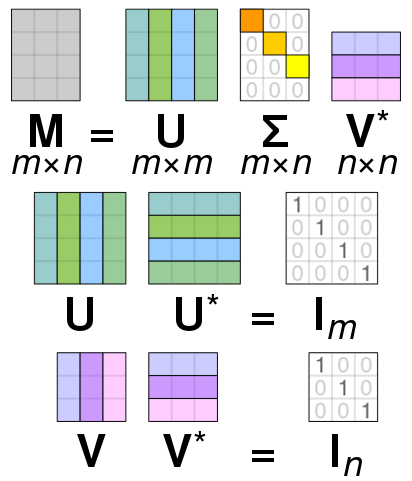
\includegraphics[width=0.5\textwidth,height=\textheight]{bilder/03-412px-Singular_value_decomposition_visualisation.svg.png}
\caption{Illustration der SVD. Bitte beachten der \(*\) bedeutet hier transponiert und komplex konjugiert. By Cmglee - Own work, CC BY-SA 4.0, \url{https://commons.wikimedia.org/w/index.php?curid=67853297}}\label{SVD}
}
\end{figure}

\hypertarget{aufgaben-1}{%
\section{Aufgaben}\label{aufgaben-1}}

Erklärung: (T) heißt theoretische Aufgabe, (P) heißt programmieren.

\hypertarget{norm-und-orthogonale-transformation-t}{%
\subsection{Norm und Orthogonale Transformation (T)}\label{norm-und-orthogonale-transformation-t}}

Sei \(Q\in \mathbb R^{n\times n}\) eine orthogonale Matrix und sei \(y\in \mathbb R^{n}\). Zeigen Sie, dass
\begin{equation*}
\|y\|^2 = \|Qy \|^2
\end{equation*}
gilt. (2 Punkte)

\hypertarget{kleinste-quadrate-und-mittelwert}{%
\subsection{Kleinste Quadrate und Mittelwert}\label{kleinste-quadrate-und-mittelwert}}

Zeigen sie, dass der \emph{kleinste Quadrate} Ansatz zur Approximation einer Datenwolke
\begin{equation*}
(x_i, y_i), \quad i=1,2,\dotsc,N,
\end{equation*}
mittels einer konstanten Funktion \(f(x)=w_1\) auf \(w_1\) auf den Mittelwert der \(y_i\) führt. (6 Punkte)

\hypertarget{qr-zerlegung-und-kleinstes-quadrate-problem-t}{%
\subsection{QR Zerlegung und Kleinstes Quadrate Problem (T)}\label{qr-zerlegung-und-kleinstes-quadrate-problem-t}}

Sei \(A\in \mathbb R^{m,n}\), \(m>n\), \(A\) hat vollen Rank und sei
\begin{equation*}
\begin{bmatrix}
Q_1 & Q_2
\end{bmatrix}
\begin{bmatrix}
\hat R \\ 0
\end{bmatrix} = A
\end{equation*}
eine QR-Zerlegung von \(A\). Zeigen sie, dass die Lösung von
\begin{equation*}
\hat R w = Q_1^T y
\end{equation*}
ein kritischer Punkt (d.h. der Gradient \(\nabla_w\) verschwindet) von
\begin{equation*}
w \mapsto \frac 12 \| Aw - y \|^2
\end{equation*}
ist. \textbf{Hinweis}: Die Formel für den Gradienten wurde in der Vorlesung 02 hergeleitet. (6 Punkte)

\hypertarget{eigenwerte-symmetrischer-matrizen-t}{%
\subsection{Eigenwerte Symmetrischer Matrizen (T)}\label{eigenwerte-symmetrischer-matrizen-t}}

Zeigen Sie, dass Eigenwerte symmetrischer reeller Matrizen \(A\in \mathbb R^{n\times n}\) immer reell sind. (3 Punkte)

\hypertarget{singuluxe4rwertzerlegung-und-eigenwerte-t}{%
\subsection{Singulärwertzerlegung und Eigenwerte (T)}\label{singuluxe4rwertzerlegung-und-eigenwerte-t}}

Zeigen Sie, dass die quadrierten Singulärwerte einer Matrix \(A\in \mathbb R^{m\times n}\), \(m>n\), genau die Eigenwerte der Matrix \(A^TA\) sind und in welcher Beziehung sie mit den Eigenwerten von \(AA^T\) stehen. \textbf{Hinweis}: hier ist ``\(m>n\)'' wichtig. (6 Punkte)

\hypertarget{python-laden-und-speichern-von-arrays}{%
\subsection{Python -- Laden und Speichern von Arrays}\label{python-laden-und-speichern-von-arrays}}

Speichern sie die Covid-Daten aus obiger Tabelle zur späteren Verwendung als ein \texttt{numpy.array}. Beispielsweise so:

\begin{Shaded}
\begin{Highlighting}[]
\ImportTok{import}\NormalTok{ numpy }\ImportTok{as}\NormalTok{ np}
\ImportTok{import}\NormalTok{ matplotlib.pyplot }\ImportTok{as}\NormalTok{ plt}

\NormalTok{days }\OperatorTok{=}\NormalTok{ [}\DecValTok{1}\NormalTok{, }\DecValTok{2}\NormalTok{, }\DecValTok{3}\NormalTok{, }\DecValTok{4}\NormalTok{, }\DecValTok{5}\NormalTok{, }\DecValTok{6}\NormalTok{, }\DecValTok{7}\NormalTok{, }\DecValTok{8}\NormalTok{, }\DecValTok{9}\NormalTok{, }\DecValTok{10}\NormalTok{, }\DecValTok{11}\NormalTok{,}
        \DecValTok{12}\NormalTok{, }\DecValTok{13}\NormalTok{, }\DecValTok{14}\NormalTok{, }\DecValTok{15}\NormalTok{,  }\DecValTok{16}\NormalTok{, }\DecValTok{17}\NormalTok{, }\DecValTok{18}\NormalTok{, }\DecValTok{19}\NormalTok{,  }\DecValTok{20}\NormalTok{,   }\DecValTok{21}\NormalTok{,}
        \DecValTok{22}\NormalTok{,  }\DecValTok{23}\NormalTok{,  }\DecValTok{24}\NormalTok{,   }\DecValTok{25}\NormalTok{,    }\DecValTok{26}\NormalTok{, }\DecValTok{27}\NormalTok{,  }\DecValTok{28}\NormalTok{,   }\DecValTok{29}\NormalTok{,    }\DecValTok{30}\NormalTok{,     }\DecValTok{31}\NormalTok{]}
\NormalTok{case }\OperatorTok{=}\NormalTok{ [}\DecValTok{352}\NormalTok{, }\DecValTok{347}\NormalTok{, }\DecValTok{308}\NormalTok{, }\DecValTok{151}\NormalTok{, }\DecValTok{360}\NormalTok{, }\DecValTok{498}\NormalTok{, }\DecValTok{664}\NormalTok{, }\DecValTok{686}\NormalTok{, }\DecValTok{740}\NormalTok{, }\DecValTok{418}\NormalTok{, }\DecValTok{320}\NormalTok{,}
        \DecValTok{681}\NormalTok{, }\DecValTok{691}\NormalTok{, }\DecValTok{1154}\NormalTok{, }\DecValTok{1284}\NormalTok{,  }\DecValTok{127}\NormalTok{, }\DecValTok{984}\NormalTok{, }\DecValTok{573}\NormalTok{, }\DecValTok{1078}\NormalTok{,  }\DecValTok{1462}\NormalTok{,   }\DecValTok{2239}\NormalTok{,}
        \DecValTok{2236}\NormalTok{,  }\DecValTok{2119}\NormalTok{,  }\DecValTok{1663}\NormalTok{,   }\DecValTok{1413}\NormalTok{,    }\DecValTok{2283}\NormalTok{,}
        \DecValTok{2717}\NormalTok{,  }\DecValTok{3113}\NormalTok{,   }\DecValTok{2972}\NormalTok{,    }\DecValTok{3136}\NormalTok{,    }\DecValTok{2615}\NormalTok{]}

\NormalTok{data }\OperatorTok{=}\NormalTok{ np.vstack([days, case])}
\BuiltInTok{print}\NormalTok{(}\StringTok{'Shape of data: '}\NormalTok{, data.shape)}

\NormalTok{datafilestr }\OperatorTok{=} \StringTok{'coviddata.npy'}
\NormalTok{np.save(datafilestr, data)}

\NormalTok{lddata }\OperatorTok{=}\NormalTok{ np.load(datafilestr)}

\NormalTok{plt.figure(}\DecValTok{1}\NormalTok{)}
\NormalTok{plt.plot(lddata[}\DecValTok{0}\NormalTok{, :], lddata[}\DecValTok{1}\NormalTok{, :], }\StringTok{'s'}\NormalTok{, label}\OperatorTok{=}\StringTok{'Cases/Day'}\NormalTok{)}
\NormalTok{plt.title(}\StringTok{'Covid Faelle in Bayern im Oktober 2020'}\NormalTok{)}
\NormalTok{plt.legend()}
\NormalTok{plt.show()}
\end{Highlighting}
\end{Shaded}

\hypertarget{lineare-regression-fuxfcr-covid-daten-p}{%
\subsection{Lineare Regression für Covid Daten (P)}\label{lineare-regression-fuxfcr-covid-daten-p}}

Führen sie auf den Covid-daten eine lineare Regression zum Fitten

\begin{itemize}
\tightlist
\item
  einer konstanten Funktion \(f(x)=c\)
\item
  einer linearen Funktion \(f(x) = ax+b\)
\item
  einer quadratischen Funktion \(f(x) = w_1 + w_2 x + w_3x^2\)
\end{itemize}

durch. Berechnen Sie die mittlere quadratische Abweichung \(\frac{1}{N}\sum_{i=1}^N\|y_i - f(x_i)\|^2\) für alle drei Approximationen und plotten Sie die Covid-Daten zusammen mit der aus der Regression erhaltenen Funktion. Beispielsweise so:

\begin{Shaded}
\begin{Highlighting}[]
\ImportTok{import}\NormalTok{ numpy }\ImportTok{as}\NormalTok{ np}
\ImportTok{import}\NormalTok{ matplotlib.pyplot }\ImportTok{as}\NormalTok{ plt}

\NormalTok{datafilestr }\OperatorTok{=} \StringTok{'coviddata.npy'}
\NormalTok{cvdata }\OperatorTok{=}\NormalTok{ np.load(datafilestr)}

\CommentTok{# ## Definieren der Basis Funktion(en)}


\KeywordTok{def}\NormalTok{ b_zero(x):}
    \CommentTok{''' eine konstante Funktion '''}
    \ControlFlowTok{return} \FloatTok{1.}


\NormalTok{ybf }\OperatorTok{=}\NormalTok{ cvdata[}\DecValTok{1}\NormalTok{, :]  }\CommentTok{# die y-werte}
\NormalTok{xbf }\OperatorTok{=}\NormalTok{ cvdata[}\DecValTok{0}\NormalTok{, :]  }\CommentTok{# die x-werte}

\NormalTok{N }\OperatorTok{=}\NormalTok{ xbf.size   }\CommentTok{# Anzahl Datenpunkte}
\NormalTok{ybf }\OperatorTok{=}\NormalTok{ ybf.reshape((N, }\DecValTok{1}\NormalTok{))  }\CommentTok{# reshape als Spaltenvektor}

\NormalTok{bzx }\OperatorTok{=}\NormalTok{ [b_zero(x) }\ControlFlowTok{for}\NormalTok{ x }\KeywordTok{in}\NormalTok{ xbf]  }\CommentTok{# eine Liste mit Funktionswerten}
\NormalTok{bzx }\OperatorTok{=}\NormalTok{ np.array(bzx).reshape((N, }\DecValTok{1}\NormalTok{))  }\CommentTok{# ein Spalten Vektor}

\NormalTok{Phix }\OperatorTok{=}\NormalTok{ bzx  }\CommentTok{# hier nur eine Spalte}

\CommentTok{# Das LGS AtA w = At y}
\NormalTok{rhs }\OperatorTok{=}\NormalTok{ Phix.T }\OperatorTok{@}\NormalTok{ ybf}
\NormalTok{AtA }\OperatorTok{=}\NormalTok{ Phix.T }\OperatorTok{@}\NormalTok{ Phix}

\CommentTok{# ACHTUNG: das hier geht nur weil AtA keine Matrix ist in diesem Fall}
\NormalTok{w }\OperatorTok{=} \FloatTok{1.}\OperatorTok{/}\NormalTok{AtA }\OperatorTok{*}\NormalTok{ rhs}
\CommentTok{# ACHTUNG: das hier ging nur weil AtA keine Matrix ist in diesem Fall}


\KeywordTok{def}\NormalTok{ get_regfunc(weights, basfunlist}\OperatorTok{=}\NormalTok{[]):}
    \CommentTok{''' Eine Funktion, die eine Funktion erzeugt}

\CommentTok{    Eingang: die Gewichte, eine Liste von Basisfunktionen}
\CommentTok{    Ausgang: die entsprechende Funktion `f = w_1b_1 + ... `}
\CommentTok{    '''}
    \KeywordTok{def}\NormalTok{ regfunc(x):}
\NormalTok{        fval }\OperatorTok{=} \DecValTok{0}
        \ControlFlowTok{for}\NormalTok{ kkk, basfun }\KeywordTok{in} \BuiltInTok{enumerate}\NormalTok{(basfunlist):}
\NormalTok{            fval }\OperatorTok{=}\NormalTok{ fval }\OperatorTok{+}\NormalTok{ weights[kkk]}\OperatorTok{*}\NormalTok{basfun(x)}
        \ControlFlowTok{return}\NormalTok{ fval}

    \ControlFlowTok{return}\NormalTok{ regfunc}


\NormalTok{const_regfunc }\OperatorTok{=}\NormalTok{ get_regfunc([w], [b_zero])}

\NormalTok{const_approx }\OperatorTok{=}\NormalTok{ [const_regfunc(x) }\ControlFlowTok{for}\NormalTok{ x }\KeywordTok{in}\NormalTok{ xbf]}
\NormalTok{const_approx }\OperatorTok{=}\NormalTok{ np.array(const_approx).reshape((N, }\DecValTok{1}\NormalTok{))}

\NormalTok{plt.figure(}\DecValTok{1}\NormalTok{)}
\NormalTok{plt.plot(cvdata[}\DecValTok{0}\NormalTok{, :], cvdata[}\DecValTok{1}\NormalTok{, :], }\StringTok{'s'}\NormalTok{, label}\OperatorTok{=}\StringTok{'Cases/Day'}\NormalTok{)}
\NormalTok{plt.plot(cvdata[}\DecValTok{0}\NormalTok{, :], const_approx, }\StringTok{'-'}\NormalTok{, label}\OperatorTok{=}\StringTok{'constant fit'}\NormalTok{)}
\NormalTok{plt.legend()}
\NormalTok{plt.show()}
\end{Highlighting}
\end{Shaded}

\textbf{Hinweise}:

\begin{itemize}
\tightlist
\item
  \texttt{liste\ =\ {[}f(x)\ for\ x\ in\ iterable{]}} ist sehr bequem um Vektoren von Funktionswerten zu erzeugen aber nicht sehr \emph{pythonesque} (und auch im Zweifel nicht effizient). Besser ist es Funktionen zu schreiben, die \emph{vektorisiert} sind. Zum Beispiel können die meisten \emph{built-in} Funktionen wie \texttt{np.exp} ein \texttt{array} als Eingang direkt in ein \texttt{array} der Funktionswerte umsetzen.
\item
  \emph{Eine Funktion, die eine Funktion erzeugt} finde ich sehr hilfreich für viele Anwendungen (ist aber manchmal nicht so gut nachvollziehbar).
\end{itemize}

\hypertarget{truncated-svd-pt}{%
\subsection{Truncated SVD (P+T)}\label{truncated-svd-pt}}

\begin{enumerate}
\def\labelenumi{\arabic{enumi}.}
\tightlist
\item
  \textbf{(P)} Berechnen und plotten sie die Singulärwerte einer \(4000\times 1000\) Matrix mit zufälligen Einträgen und die einer Matrix mit ``echten'' Daten (hier Simulationsdaten einer Stroemungssimulation)\footnote{\href{https://owncloud.gwdg.de/index.php/s/sAjEy9B8kIbzoYj}{Download bitte hier} -- Achtung das sind 370MB}. Berechnen sie den Fehler der \emph{truncated SVD} \(\|A-A_{\hat r}\|\) für \(\hat r = 10, 20, 40\) für beide Matrizen.
\item
  \textbf{(T)} Was lässt sich bezüglich einer Kompression der Daten mittels SVD für die beiden Matrizen sagen. (Vergleichen sie die plots der Singulärwerte und beziehen sie sich auf die gegebene Formel für die Differenz).
\item
  \textbf{(P+T)} Für die ``echten'' Daten: Speichern sie die Faktoren der bei \(\hat r=40\) abgeschnittenen SVD und vergleichen Sie den Speicherbedarf der Faktoren und der eigentlichen Matrix.
\end{enumerate}

Beispielcode:

\begin{Shaded}
\begin{Highlighting}[]
\ImportTok{import}\NormalTok{ numpy }\ImportTok{as}\NormalTok{ np}
\ImportTok{import}\NormalTok{ scipy.linalg }\ImportTok{as}\NormalTok{ spla}
\ImportTok{import}\NormalTok{ matplotlib.pyplot }\ImportTok{as}\NormalTok{ plt}

\NormalTok{randmat }\OperatorTok{=}\NormalTok{ np.random.randn(}\DecValTok{4000}\NormalTok{, }\DecValTok{1000}\NormalTok{)}

\NormalTok{rndU, rndS, rndV }\OperatorTok{=}\NormalTok{ spla.svd(randmat)}

\BuiltInTok{print}\NormalTok{(}\StringTok{'U-dims: '}\NormalTok{, rndU.shape)}
\BuiltInTok{print}\NormalTok{(}\StringTok{'V-dims: '}\NormalTok{, rndV.shape)}
\BuiltInTok{print}\NormalTok{(}\StringTok{'S-dims: '}\NormalTok{, rndS.shape)}

\NormalTok{plt.figure(}\DecValTok{1}\NormalTok{)}
\NormalTok{plt.semilogy(rndS, }\StringTok{'.'}\NormalTok{, label}\OperatorTok{=}\StringTok{'Singulaerwerte (random Matrix)'}\NormalTok{)}

\NormalTok{realdatamat }\OperatorTok{=}\NormalTok{ np.load(}\StringTok{'velfielddata.npy'}\NormalTok{)}

\CommentTok{# # Das hier ist eine aufwaendige Operation}
\NormalTok{rlU, rlS, rlV }\OperatorTok{=}\NormalTok{ spla.svd(realdatamat, full_matrices}\OperatorTok{=}\VariableTok{False}\NormalTok{)}
\CommentTok{# # auf keinen Fall `full_matrices=False` vergessen}

\BuiltInTok{print}\NormalTok{(}\StringTok{'U-dims: '}\NormalTok{, rlU.shape)}
\BuiltInTok{print}\NormalTok{(}\StringTok{'V-dims: '}\NormalTok{, rlV.shape)}
\BuiltInTok{print}\NormalTok{(}\StringTok{'S-dims: '}\NormalTok{, rlS.shape)}

\NormalTok{plt.figure(}\DecValTok{1}\NormalTok{)}
\NormalTok{plt.semilogy(rlS, }\StringTok{'.'}\NormalTok{, label}\OperatorTok{=}\StringTok{'Singulaerwerte (Daten Matrix)'}\NormalTok{)}

\NormalTok{plt.legend()}
\NormalTok{plt.show()}
\end{Highlighting}
\end{Shaded}

\textbf{Hinweise}:

\begin{itemize}
\tightlist
\item
  Es gibt viele verschiedene Normen für Vektoren und Matrizen. Sie dürfen einfach mit \texttt{np.linalg.norm} arbeiten. Gerne aber mal in die Dokumentation schauen \emph{welche} Norm berechnet wird.
\item
  Die (T) Abschnitte hier bitte mit den anderen (T) Aufgaben oder als Bildschirmausgabe im Programm.
\end{itemize}

\hypertarget{hauptkomponentenanalyse}{%
\chapter{Hauptkomponentenanalyse}\label{hauptkomponentenanalyse}}

Während in den vorherigen Kapiteln der Versuch war, einen funktionalen Zusammenhang in Daten zu bekommen, geht es jetzt darum, statistische Eigenschaften aus Daten zu extrahieren. Wir werden sehen, dass das auch nur ein anderer Blickwinkel auf das gleiche Problem \emph{Wie können wir die Daten verstehen?} ist und auch die SVD wieder treffen.

Weil ich den Ansatz gerne \emph{ad hoc} also am Problem entlang motivieren und einführen will, vorweg schon mal die bevorstehenden Schritte

\begin{enumerate}
\def\labelenumi{\arabic{enumi}.}
\tightlist
\item
  Zentrierung/Skalierung der Daten
\item
  Berechnung der Varianzen im Standard Koordinatensystem
\item
  Überlegung, dass Daten in einem anderen Koordinatensystem eventuell besser dargestellt werden im Sinne
\item
  Berechnung eines optimalen Koordinatenvektors mittels SVD.
\end{enumerate}

Wir nehmen noch einmal die Covid-Daten her, vergessen kurz, dass es sich um eine Zeitreihe handelt und betrachten sie als Datenpunkte \((x_i, y_i)\), \(i=1,\dotsc,N\), im zweidimensionalen Raum mit Koordinaten \(x\) und \(y\).

Als erstes werden die Daten \textbf{zentriert} indem in jeder Komponente der Mittelwert
\begin{equation*}
x_c = \frac 1N \sum_{i=1}^N x_i,
\quad
y_c = \frac 1N \sum_{i=1}^N y_i.
\end{equation*}
abgezogen wird und dann noch mit dem inversen des Mittelwerts skaliert.

Also, die Daten werden durch \((\frac{x_i-\bar x}{\bar x},\, \frac{y_i-\bar y}{\bar y})\) ersetzt.

\begin{figure}
\hypertarget{fig:cases-cntrd}{%
\centering
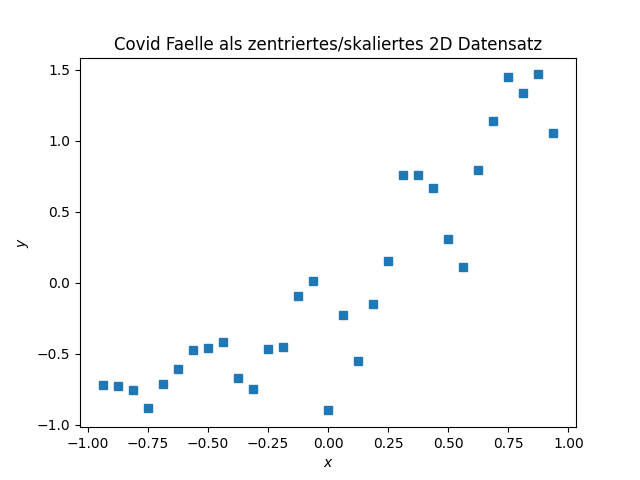
\includegraphics[width=0.65\textwidth,height=\textheight]{bilder/04-covid-cntrd.png}
\caption{Fallzahlen von Sars-CoV-2 in Bayern im Oktober
2020 -- zentriert}\label{fig:cases-cntrd}
}
\end{figure}

\hypertarget{variationskoeffizienten}{%
\section{Variationskoeffizienten}\label{variationskoeffizienten}}

Als nächstes kann Jan sich fragen, wie gut die Daten durch ihren Mittelwert beschrieben werden und die Varianzen berechnen, die für zentrierte Daten so aussehen

\begin{equation*}
s_x^2 = \frac {1}{N-1} \sum_{i=1}^N x_i^2,
\quad
s_y^2 = \frac {1}{N-1} \sum_{i=1}^N y_i^2.
\end{equation*}

Im gegebenen Fall bekommen wir
\begin{equation*}
s_x^2 \approx 0.32
\quad
s_y^2 \approx  0.57
\end{equation*}
und schließen daraus, dass in \(y\) Richtung \emph{viel passiert} und in \(x\) Richtung \emph{nicht ganz so viel}. Das ist jeder Hinsicht nicht befriedigend, wir können weder

\begin{itemize}
\tightlist
\item
  Redundanzen ausmachen (eine Dimension der Daten vielleicht weniger wichtig?) noch
\item
  dominierende Richtungen feststellen (obwohl dem Bild nach so eine offenbar existiert)
\end{itemize}

und müssen konstatieren, dass die Repräsentation der Daten im \((x,y)\) Koordinatensystem nicht optimal ist.

Die Frage ist also, ob es ein Koordinatensystem gibt, dass die Daten besser darstellt.

\leavevmode\hypertarget{rem-coors}{}%
\begin{JHSAYS}
Ein Koordinatensystem ist nichts anderes als eine Basis. Und die Koordinaten eines Datenpunktes sind die Komponenten des entsprechenden Vektors in dieser Basis. Typischerweise sind Koordinatensysteme orthogonal (das heißt eine Orthogonalbasis) und häufig noch orientiert (die Basisvektoren haben eine bestimmte Reihenfolge und eine bestimmte Richtung).

\end{JHSAYS}

\hypertarget{koordinatenwechsel}{%
\section{Koordinatenwechsel}\label{koordinatenwechsel}}

Sei nun also \(\{b_1,b_2\}\subset \mathbb R^{2}\) eine orthogonale Basis.

\leavevmode\hypertarget{rem-ortho-bas}{}%
\begin{JHSAYS}
Wie allgemein gebräuchlich, sagen wir \emph{orthogonal}, meinen aber \emph{orthonormal}. In jedem Falle soll gelten
\begin{equation*}
b_1^T b_1=1, \quad b_2^Tb_2=1, \quad b_1^Tb_2 = b_2^Tb_1 = 0.
\end{equation*}

\end{JHSAYS}

Wir können also alle Datenpunkte
\(\mathbf x_i = \begin{bmatrix} x_i \\ y_i \end{bmatrix}\)
in der neuen Basis darstellen mit eindeutig bestimmten Koeffizienten \(\alpha_{i1}\) und \(\alpha_{i2}\) mittels
\begin{equation*}
\mathbf x_i = \alpha_{i1}b_1 + \alpha_{i2}b_2.
\end{equation*}
Für orthogonale Basen sind die Koeffizienten durch \emph{testen} mit dem Basisvektor einfach zu berechnen:
\begin{align*}
b_1^T\mathbb x_i = b_1^T(\alpha_{i1}b_1 + \alpha_{i2}b_2) = \alpha_{i1}b_1^Tb_1 + \alpha_{i2}b_1^Tb_2 = \alpha_{i1}\cdot 1 + \alpha_{i2} \cdot 0 = \alpha_{i1},\\
b_2^T\mathbb x_i = b_2^T(\alpha_{i1}b_1 + \alpha_{i2}b_2) = \alpha_{i1}b_1^Tb_2 + \alpha_{i2}b_2^Tb_2 = \alpha_{i1}\cdot 0 + \alpha_{i2}\cdot 1 = \alpha_{i2}.
\end{align*}
Es gilt also
\begin{equation*}
\alpha_{i1} = b_1^T\mathbb x = b_1^T\begin{bmatrix}
x_i \\ y_i
\end{bmatrix}, \quad
\alpha_{i2} = b_2^T\mathbb x = b_2^T\begin{bmatrix}
x_i \\ y_i
\end{bmatrix}.
\end{equation*}

Damit, können wir jeden Datenpunkt \(\mathbf x_i=(x_i, y_i)\) in den neuen Koordinaten \((\alpha_{i1}, \alpha_{i2})\) ausdrücken.

Zunächst halten wir fest, dass auch in den neuen Koordinaten die Daten zentriert sind. Es gilt nämlich, dass
\begin{equation*}
\frac 1N \sum_{i=1}^N \alpha_{ji}=\frac 1N \sum_{i=1}^N b_j^T\mathbb x_i 
=\frac 1N b_j^T \sum_{i=1}^N \begin{bmatrix} x_i \\ y_i \end{bmatrix}
=\frac 1N b_j^T \begin{bmatrix} \sum_{i=1}^N x_i \\ \sum_{i=1}^N y_i \end{bmatrix}
=b_j^T \begin{bmatrix} \frac 1N \sum_{i=1}^N x_i \\ \frac 1N \sum_{i=1}^N y_i \end{bmatrix}
=b_j^T \begin{bmatrix} 0 \\ 0 \end{bmatrix} = 0,
\end{equation*}
für \(j=1,2\).

Desweiteren gilt wegen der Orthogonalität von \(B=[b_1~b_2]\in \mathbb R^{2\times 2}\), dass
\begin{equation*}
x_{i}^2 + y_{i}^2 = \|\mathbb x_i\|^2 = \|B^T\mathbb x_i\|^2 
= \|\begin{bmatrix} b_1^T \\ b_2^T \end{bmatrix} \mathbb x_i\|^2
= \|\begin{bmatrix} b_1^T\mathbb x \\ b_2^T\mathbb x \end{bmatrix}\|^2
= \|\begin{bmatrix} \alpha_{i1} \\ \alpha_{i2} \end{bmatrix}\|^2
= \alpha_{i1}^2 + \alpha_{i2}^2
\end{equation*}
woraus wir folgern, dass in jedem orthogonalen Koordinatensystem, die Summe der beiden Varianzen die gleiche ist:
\begin{equation*}
s_x^2 + s_y^2 = \frac{1}{N-1}\sum_{i=1}^N(x_i^2 + y_i^2) = \frac{1}{N-1}\sum_{i=1}^N(\alpha_{i1}^2 + \alpha_{i2}^2) =: s_1^2 + s_2^2.
\end{equation*}

Das bedeutet, dass durch die Wahl des Koordinatensystems die Varianz als Summe nicht verändert wird. Allerdings können wir das System so wählen, dass eine der Varianzen in Achsenrichtung maximal wird (und die übrige(n) entsprechend klein).

Analog gilt für den eigentlichen Mittelwert der (nichtzentrierten) Daten, dass die Norm gleich bleibt. In der Tat, für die \emph{neuen} Koordinaten des Mittelwerts gilt in der Norm
\begin{equation*}
\|
\begin{bmatrix}
\alpha_{c1} \\ \alpha_{c2}
\end{bmatrix}
\|
=
\|
B^T
\begin{bmatrix}
x_c \\ y_c
\end{bmatrix}
\|
=
\|
\begin{bmatrix}
x_c \\ y_c
\end{bmatrix}
\|.
\end{equation*}

\hypertarget{maximierung-der-varianz-in-haupt-achsenrichtung}{%
\section{Maximierung der Varianz in (Haupt)-Achsenrichtung}\label{maximierung-der-varianz-in-haupt-achsenrichtung}}

Wir wollen nun also \(b_1\in \mathbb R^{2}\), mit \(\|b_1\|=1\) so wählen, dass
\begin{equation*}
s_1^2 = \frac{1}{N-1}\sum_{i=1}^n \alpha_{i1}^2
\end{equation*}
maximal wird. Mit der Matrix \(\mathbf X\) aller Daten
\begin{equation*}
\mathbf X = \begin{bmatrix}
x_1 & y_1 \\ x_2 & y_2 \\ \vdots & \vdots \\ x_N & y_N
\end{bmatrix} = 
\begin{bmatrix}
\mathbf x_1^T\\ \mathbf x_2^T  \\  \vdots \\ \mathbf x_N^T
\end{bmatrix} 
\in \mathbb R^{N\times 2}
\end{equation*}
können wir die Varianz in \(b_1\)-Richtung kompakt schreiben als
\begin{equation*}
s_1^2 = \frac{1}{N-1}\sum_{i=1}^n \alpha_{i1}^2
= \frac{1}{N-1}\sum_{i=1}^n (b_1^T\mathbf x_i)^2
= \frac{1}{N-1}\sum_{i=1}^n (\mathbf x_i^Tb_1)^2
= \frac{1}{N-1}\| \mathbf X b_1 \|^2
\end{equation*}
Wir sind also ein weiteres mal bei einem Optimierungsproblem (diesmal mit Nebenbedingung) angelangt:
\begin{equation*}
\max_{b\in \mathbb R^{2},\, \|b\|=1} \|\mathbf X b\|^2
\end{equation*}
Die Lösung dieses Problems ist mit \(b=v_1\) gegeben, wobei \(v_1\) der erste (rechte) Singulärvektor von \(\mathbf X\) ist:
\begin{equation*}
\mathbf X = U \Sigma V^T = U \Sigma \begin{bmatrix}
v_1^T \\ v_2^T
\end{bmatrix}.
\end{equation*}
Und damit rechnen wir auch direkt nach, dass im neuen Koordinatensystem \(\{b_1, b_2\}=\{v_1, v_2\}\) die Varianzen \(s_1^2\) und \(s_2^2\) (bis auf einen Faktor von \(\frac{1}{N-1}\)) genau die quadrierten Singulärwerte von \(\mathbf X\) sind:
\begin{align*}
(N-1)s_1^2 
= \|\mathbf X v_1 \|^2 = \|U \Sigma \begin{bmatrix} v_1^T \\ v_2^T \end{bmatrix}v_1\|^2
= \|\Sigma \begin{bmatrix} v_1^Tv_1 \\ v_2^T v_1\end{bmatrix}\|^2
=  \|\Sigma \begin{bmatrix} 1 \\  0\end{bmatrix}\|^2
=\sigma_1^2,\\
(N-1)s_2^2 
= \|\mathbf X v_2 \|^2 = \|U \Sigma \begin{bmatrix} v_1^T \\ v_2^T \end{bmatrix}v_2\|^2
= \|\Sigma \begin{bmatrix} v_1^Tv_2 \\ v_2^T v_2\end{bmatrix}\|^2
=  \|\Sigma \begin{bmatrix} 0 \\  1\end{bmatrix}\|^2
=\sigma_2^2
\end{align*}

Für unser Covid Beispiel ergibt sich
\begin{equation*}
V^T \approx
\begin{bmatrix}
0.5848 &  0.8111 \\
0.8111 & -0.5848
\end{bmatrix}
\end{equation*}
also
\begin{equation*}
b_1 = v_1 = \begin{bmatrix}
0.5848 \\  0.8111 
\end{bmatrix}
\quad
b_2 = v_2 = \begin{bmatrix}
0.8111 \\ -0.5848
\end{bmatrix}
\end{equation*}
als neue Koordinatenrichtungen mit
\begin{equation*}
s_1^2 \approx 0.85, \quad s_2^2 \approx 0.04,
\end{equation*}
was bereits eine deutliche Dominanz der \(v_1\)-Richtung -- genannt \emph{Hauptachse} -- zeigt.

Im Hinblick auf die nächste Vorlesung, in der wir Anwendungen und Eigenschaften der PCA untersuchen werden, noch ein Plot der Daten mit der \(v_1\)-Richtung als Linie eingezeichnet.

\begin{figure}
\hypertarget{fig:cases-cntrd-HA}{%
\centering
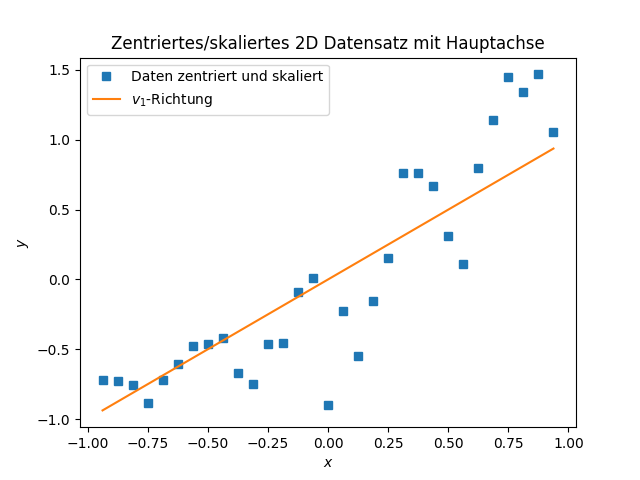
\includegraphics[width=0.65\textwidth,height=\textheight]{bilder/04-covid-cntrd-HA.png}
\caption{Fallzahlen von Sars-CoV-2 in Bayern im Oktober
2020 -- zentriert/skaliert/Hauptachse}\label{fig:cases-cntrd-HA}
}
\end{figure}

\hypertarget{hauptkomponentenanalyse-ctd.}{%
\chapter{Hauptkomponentenanalyse Ctd.}\label{hauptkomponentenanalyse-ctd.}}

\newcommand{\Cov}{\operatorname{Cov}}
\newcommand{\bX}{{\mathbf{X}}}
\newcommand{\bxi}{{\mathbf{x} _ i}}
\newcommand{\bxj}{{\mathbf{x} _ j}}
\newcommand{\bxixj}{{\mathbf{x} _ i \mathbf{x} _ j}}

Im vorherigen Kapitel hatten wir einen zweidimensionalen Datensatz betrachtet und dafür die Richtung bestimmt, in der die Varianz maximal wird.
Da wir außerdem ermittelt hatten, dass die Summe der Varianz unabhüngig vom Koordinatensystem ist (es muss nur ein orthogonales sein) bedeutete das gleichzeitig, dass die verbleibende Richtung die Richtung der minimalen Varianz war.

Jetzt wollen wir einen Datensatz mit mehr Merkmalen betrachten und sehen, wie die algorithmische Herangehensweise zum Verständnis beiträgt.

\hypertarget{der-penguins-datensatz}{%
\section{Der PENGUINS Datensatz}\label{der-penguins-datensatz}}

Die Grundlage ist der \href{https://allisonhorst.github.io/palmerpenguins/}{\emph{Pinguin Datensatz}}, der eine gern genommene Grundlage für die Illustration in der Datenanalyse ist. Die Daten wurden von \href{https://www.uaf.edu/cfos/people/faculty/detail/kristen-gorman.php}{Kristen Gorman} erhoben und beinhalten 4 verschiedene Merkmale (engl. \emph{features}) von einer Stichprobe von insgesamt 344\footnote{allerdings mit 2 unvollsändigen Datenpunkten, die ich entfernt habe für unseere Beispiele}Pinguinen die 3 verschiedenen Spezies zugeordnet werden können oder sollen (Fachbegriff hier: \emph{targets}). Im Beispiel werden die Klassen mit \texttt{0,\ 1,\ 2} codiert und beschreiben die Unterarten \emph{Adele}, \emph{Gentoo} und \emph{Chinstrap} der Schwertlilien. Die Merkmale sind gemessene Länge und Höhe des Schnabels (hier \emph{bill}), die Länge der Flosse (\emph{flipper}) sowie das Köpergewicht \footnote{Im Originaldatensatz ist das Gewicht in Gramm angegeben, um die Daten innerhalb einer 10er Skala zu haben, habe ich das Gewicht auf in kg umgerechnet}
(\emph{body mass}).

Wir stellen uns 2-3 Fragen:

\begin{enumerate}
\def\labelenumi{\arabic{enumi}.}
\tightlist
\item
  Würden eventuell 3 (oder sogar nur 2) Dimensionen reichen um den Datensatz zu beschreiben?
\item
  Können wir aus den Merkmalen (\emph{features}) die Klasse (\emph{target}) erkennen und wie machen wir gegebenenfalls die Zuordnung?
\end{enumerate}

\hypertarget{darstellung}{%
\section{Darstellung}\label{darstellung}}

In höheren Dimensionen ist schon die graphische Darstellung der Daten ein Problem. Wir können aber alle möglichen 2er Kombinationen der Daten in 2D plots visualisieren.

\begin{figure}
\hypertarget{fig:05-penguin-allpairs}{%
\centering
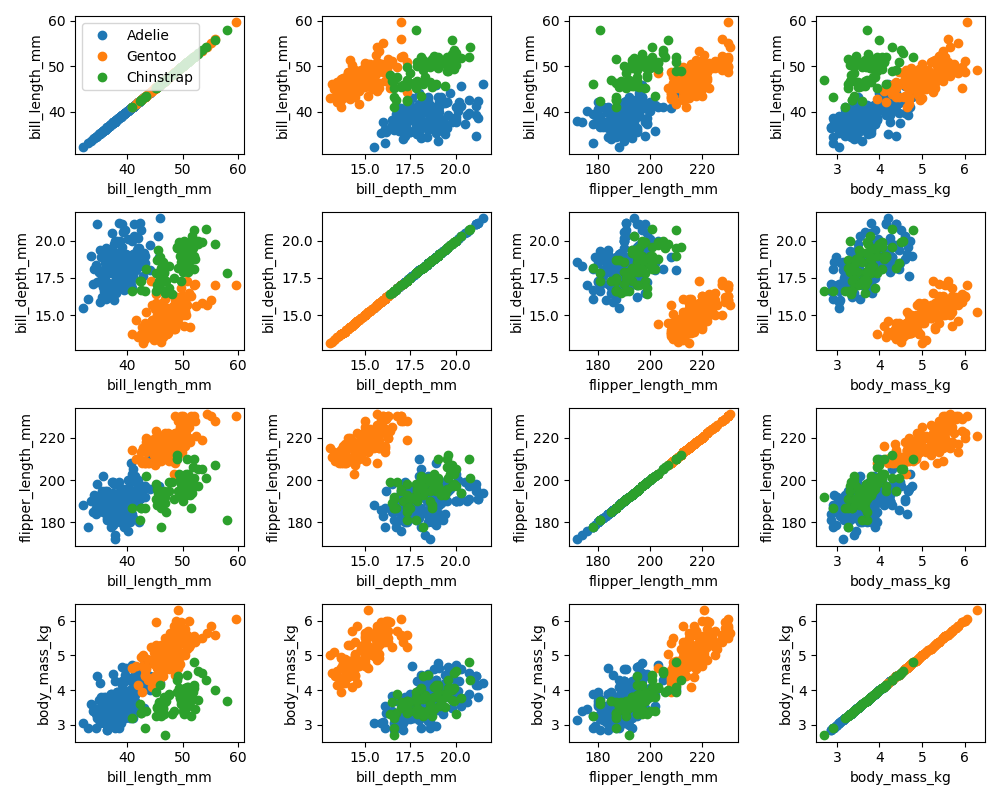
\includegraphics[width=0.75\textwidth,height=\textheight]{bilder/05-all-pairs.png}
\caption{Pinguin Datenset 2D plots}\label{fig:05-penguin-allpairs}
}
\end{figure}

Ein Blick auf die Diagonale zeigt schon, dass manche Merkmale besser geeignet als andere sind, um die Spezies zu unterscheiden, allerdings keine der Zweierkombinationen eine Eindeutige Diskriminierung erlaubt.

\hypertarget{korrelationen-und-die-kovarianzmatrix}{%
\section{Korrelationen und die Kovarianzmatrix}\label{korrelationen-und-die-kovarianzmatrix}}

Als nächstes suchen wir nach Korrelationen in den Daten in dem wir für alle Merkmalpaare die Korrelationen ausrechnen. Dafür berechnen wir die sogenannte \emph{Kovarianzmatrix}
\begin{equation*}
\operatorname{Cov}(\mathbf X) = \begin{bmatrix}
\rho_{{\mathbf{x} _ i \mathbf{x} _ j}}
\end{bmatrix}_{i,j=1,\dots n} \in \mathbb R^{n\times n}
\end{equation*}
wobei \(n\) die Dimension der Daten ist und wobei
\begin{equation*}
s_{{\mathbf{x} _ i \mathbf{x} _ j}} = \frac{1}{N-1} \sum_{k=1}^N (x_{ik}-\overline{{\mathbf{x} _ i}})(x_{jk}-\overline{{\mathbf{x} _ j}} ).
\end{equation*}
die Kovarianzen sind, die wir auch schon in der ersten Vorlesung kennengelernt haben.

Ist \(\mathbf X\in \mathbb R^{N\times n}\) die Matrix mit den Datenvektoren \({\mathbf{x} _ i}\in \mathbb R^{n}\) als Spalten \textbf{und ist der Datensatz zentriert} so erhalten wir die Kovarianzmatrix als
\begin{equation*}
\operatorname{Cov}({\mathbf{X}}) = \frac{1}{N-1}{\mathbf{X}}^T {\mathbf{X}}
\end{equation*}

Wir bemerken, dass auf der Hauptdiagonalen die Varianzen in Koordinatenrichtung stehen und in den Zeilen oder Spalten ein Mass dafür, wie bspw. \({\mathbf{x} _ i}\) und \({\mathbf{x} _ j}\) korreliert sind. Große Zahlen bedeuten eine große Varianz oder eine starke Korrelation und umgekehrt. Für die Datenanalyse können wir \(\operatorname{Cov}({\mathbf{X}})\) wie folgt heranziehen:

\hypertarget{hauptachsentransformation}{%
\section{Hauptachsentransformation}\label{hauptachsentransformation}}

Wie im vorherigen Kapitel hergeleitet, bedeutet ein Koordinatenwechsel die Multiplikation der Datenmatrix \({\mathbf{X}}\in \mathbb R^{N\times n}\) mit einer orthogonalen
Matrix \(V\in \mathbb R^{n\times n}\):
\begin{equation*}
\tilde {\mathbf{X}}= {\mathbf{X}}V,
\end{equation*}
wobei \(\tilde {\mathbf{X}}\) die Daten in den neuen Koordinaten sind (die Basisvektoren sind dann die Zeilenvektoren von \(V\)). Wir wollen nun eine Basis finden, in der

\begin{itemize}
\tightlist
\item
  \(\operatorname{Cov}({\mathbf{X}})\) eine Diagonalmatrix ist --- damit wären alle Richtungen in den Daten \emph{unkorreliert} und könnten \emph{unabhängig} voneinander betrachtet werden\footnote{wir dürfen aber nicht vergessen, dass Daten tüpischerweise nur eine Stichprobe von Beobachtungen eines Phänomens sind. Die Unabhängigkeit in den \emph{features} gilt also nur für die gesammelten Daten aber in der Regel nicht für das Phänomen. Für normalverteilte Prozesse liefern die daten-basiert ermittelten Hauptrichtungen jedoch auch die Hauptrichtungen des zugrundeliegenden Phänomens} --
\item
  und in der die neuen Varianzen nach Größe geordnet sind gleichzeitig die verfügbare Varianz maximal in wenigen Richtungen konzentrieren.
\end{itemize}

Nachden den Überlegungen im vorherigen Kapitel ist die erste Hauptrichtung durch den ersten rechten Singulärvektor \(v_1\in \mathbb R^{n}\) der (\emph{ökonomischen}) Singulärwertzerlegung
\begin{equation*}
{\mathbf{X}}= U\Sigma V^* = 
\begin{bmatrix}
u_1 & u_2 & \dots & u_n
\end{bmatrix}
\begin{bmatrix}
\sigma_1 \\ &\sigma_2 \\ &&\ddots \\ &&&\sigma_n
\end{bmatrix}
\begin{bmatrix}
v_1^* \\ v_2 ^* \\ \vdots \\ v_n^*
\end{bmatrix}
\end{equation*}
von \(\mathbf X\in \mathbb R^{N\times n}\) gegeben. Die zugehörigen Koeffizenten berechnen wir mittels
\begin{equation*}
\tilde {\mathbf{X}}= {\mathbf{X}}v_1.
\end{equation*}

\hypertarget{rekonstruktion}{%
\section{Rekonstruktion}\label{rekonstruktion}}

Um zu plausibilisieren, dass die weiteren Hauptachsen durch die weiteren (rechten) Singulärvektoren gegeben sind, betrachten wir erst die \emph{Rekonstruktion}
also die Darstellung im Ausgangskoordinatensystem (mit den messbaren oder interpretierbaren Features) die durch
\begin{equation*}
\tilde {\tilde {\mathbf{X}}} = {\mathbf{X}}v_1v_1^T
\end{equation*}
gegeben ist.
Die letzte Formel wird vielleicht klarer, wenn Jan sich überlegt, dass für einen Datenpunkt \({\mathbf{X}}_j=\begin{bmatrix} x_{1j} &x_{2j} & \dots& x_{nj}\end{bmatrix}\) (also die \(j\)-te Zeile von \({\mathbf{X}}\)), der Koeffizient für \(v_1\) gegeben ist durch \(\alpha_j=v_1^T{\mathbf{X}}_j^T\) und die Darstellung im Vektorraum durch
\begin{equation*}
\tilde{\tilde{ {\mathbf{X}}}}_j=(\alpha_j v_1)^T = \alpha_j v_1^T = (v_1^T {\mathbf{X}}_j^T) v_1^T  = {\mathbf{X}}_j  v_1 v_1^T
\end{equation*}
gegeben ist.

Damit können wir mit
\begin{equation*}
{\mathbf{X}}- \tilde{\tilde {{\mathbf{X}}}} = {\mathbf{X}}(I-v_1v_1^T)
\end{equation*}
den Teil der Daten betrachten, der durch die Richtung \(v_1\) nicht abgebildet wird (sozusagen den noch verbleibenden Teil). Jan kann nachrechnen, dass wiederum \(U\) und \(V\) die Singulärvektoren von \({\mathbf{X}}-\tilde{\tilde {{\mathbf{X}}}}\) bilden, mit jetzt \(v_2\) als Richtung mit dem größten (verbleibenden) Singulärwert.

Das heißt, dass der \(k\)-te Singulärvektor die \(k\)-te Hauptrichtung bildet.

\hypertarget{reduktion-der-daten}{%
\section{Reduktion der Daten}\label{reduktion-der-daten}}

Ist die Datenmatrix mit linear abhängigen Spalten besetzt, äußert sich das in \(\sigma_k = 0\) für ein \(k<n\) (und alle noch folgenden Singulärwerte). Jan rechnet nach, dass dann
\begin{equation*}
{\mathbf{X}}= {\mathbf{X}}V_{k-1}V_{k-1}^T
\end{equation*}
wobei \(V_{k-1}\) die Matrix der \(k-1\) führenden Singulärvektoren ist und das entsprechende
\begin{equation*}
\tilde {\mathbf{X}}= {\mathbf{X}}V_{k-1}
\end{equation*}
alle Informationen des Datensatzes in kleinerer Dimension parametrisiert.

In der Praxis sind schon allein durch Messfehler exakte lineare Abhängigkeiten sowie durch die näherungsweise Bestimmung auf dem Computer das Auftreten von \(\sigma_k =0\) quasi ausgeschlossen. Stattdessen werden Schwellwerte definiert, unterhalb derer die SVD abgeschnitten wird.

Wie oben, werden dann die Daten \(\tilde {\mathbf{X}}={\mathbf{X}}V_{\hat k}\) in den (reduzierten) Koordinaten der Hauptachsen betrachtet sowie die Rekonstruktion \(\hat {\mathbf{X}}= {\mathbf{X}}V_{\hat k}V_{\hat k}^T\), wobei der \(V_{\hat k}\) die Matrix der \(\hat k\) führenden Singulärvektoren sind (mit Singulärwerten überhalb des Schwellwertes).

\hypertarget{am-beispiel-der-pinguin-daten}{%
\section{Am Beispiel der Pinguin Daten}\label{am-beispiel-der-pinguin-daten}}

Wir stellen die Daten noch einmal zentriert dar:

\begin{figure}
\hypertarget{fig:05-penguin-allpairs-cntrd}{%
\centering
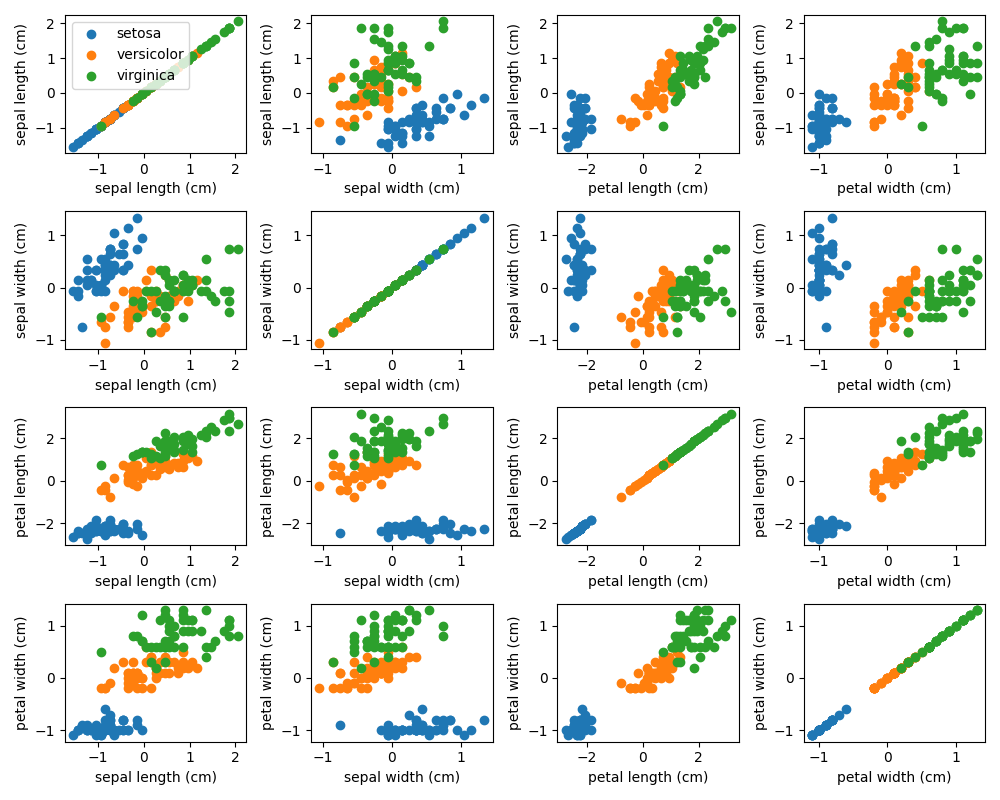
\includegraphics[width=0.75\textwidth,height=\textheight]{bilder/05-all-pairs-cntrd.png}
\caption{Pinguin Daten Zentriert}\label{fig:05-penguin-allpairs-cntrd}
}
\end{figure}

Für die Kovarianzmatrix der Pinguin Daten erhalten wir:

\begin{Shaded}
\begin{Highlighting}[]
\NormalTok{Covariance matrix: }
\NormalTok{[[ }\FloatTok{29.8071}  \FloatTok{-2.5342}  \FloatTok{50.3758}   \FloatTok{2.6056}\NormalTok{]}
\NormalTok{ [ }\FloatTok{-2.5342}   \FloatTok{3.8998} \FloatTok{-16.213}   \FloatTok{-0.7474}\NormalTok{]}
\NormalTok{ [ }\FloatTok{50.3758} \FloatTok{-16.213}  \FloatTok{197.7318}   \FloatTok{9.8244}\NormalTok{]}
\NormalTok{ [  }\FloatTok{2.6056}  \FloatTok{-0.7474}   \FloatTok{9.8244}   \FloatTok{0.6431}\NormalTok{]]}
\end{Highlighting}
\end{Shaded}

Für die Singulärwerte:

\begin{Shaded}
\begin{Highlighting}[]
\NormalTok{In: U, S, Vh }\OperatorTok{=}\NormalTok{ np.linalg.svd(data, full_matrices}\OperatorTok{=}\VariableTok{False}\NormalTok{)}

\NormalTok{In: }\BuiltInTok{print}\NormalTok{(S)}
\NormalTok{Out: [}\FloatTok{269.7858}  \FloatTok{74.1334}  \FloatTok{28.4183}   \FloatTok{7.2219}\NormalTok{]}
\end{Highlighting}
\end{Shaded}

Zwar ist hier kein Singulärwert nah an der Null, allerdings beträgt der Unterschied zwischen dem größten und dem kleinsten schon eine gute 10er Potenz, was auf eine starke Dominanz der ersten Hauptachsen hinweist.

In der Tat, plotten wir die Daten in den Koordinaten der Hauptachsen (also \(\tilde {\mathbf{X}}\)), zeigen Bilder der \(v_1\) oder \(v_2\)-Koordinaten klare Tendenzen in den Daten, während die Plots der übrigen Richtungen wie eine zufällige Punktwolke aussieht, vgl. Abbildung \ref{fig:05-penguin-allpairs-pcs}.

\begin{figure}
\hypertarget{fig:05-penguin-allpairs-pcs}{%
\centering
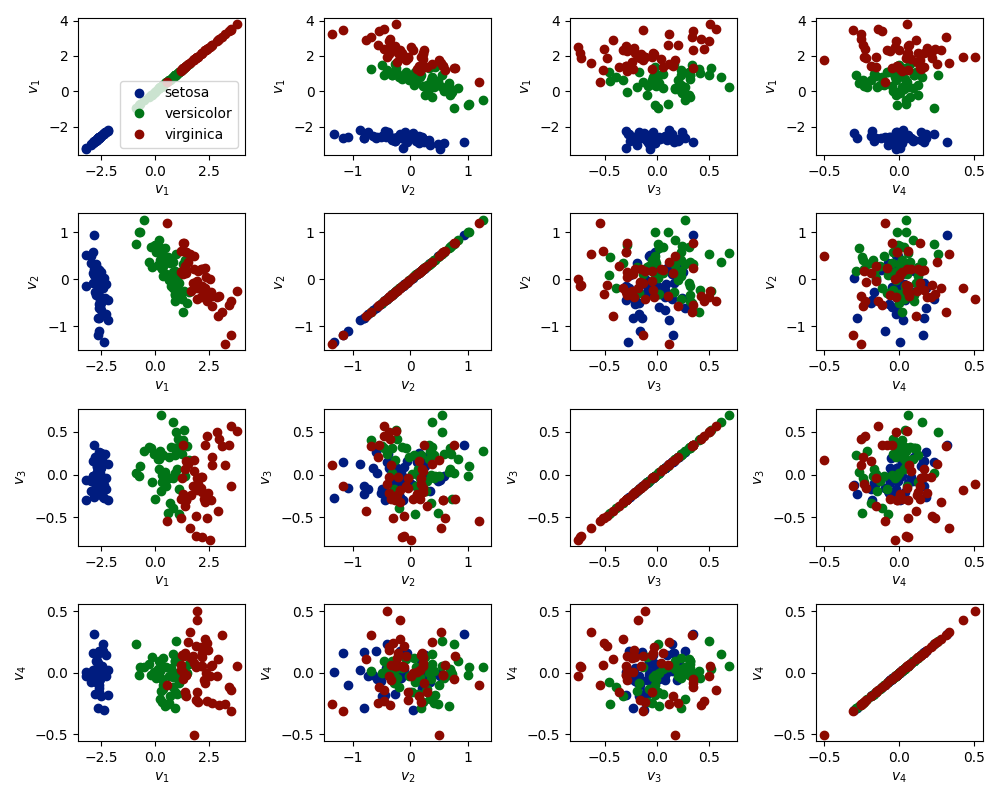
\includegraphics[width=0.75\textwidth,height=\textheight]{bilder/05-all-pairs-pcs.png}
\caption{Pinguin Datenset 2D plots in Hauptachsenkoordinaten}\label{fig:05-penguin-allpairs-pcs}
}
\end{figure}

Als letztes plotten wir noch \(\hat {{\mathbf{X}}}\) für \(\hat k =2\). Das heißt wir reduzieren die Daten auf die \(v_1\) und \(v_2\)-Richtungen und betrachten die Rekonstruktion. Im Plot sehen wir, dass in gewissen Teilen die Daten gut rekonstruiert werden. Allerdings, hat \(\hat{{\mathbf{X}}}\) nur Rang \(\operatorname{Rk} \hat {{\mathbf{X}}}=2\) (warum?), sodass in den Plots notwendigerweise direkte lineare Abhängigkeiten offenbar werden.

\begin{figure}
\hypertarget{fig:05-penguin-allpairs-k2-rec}{%
\centering
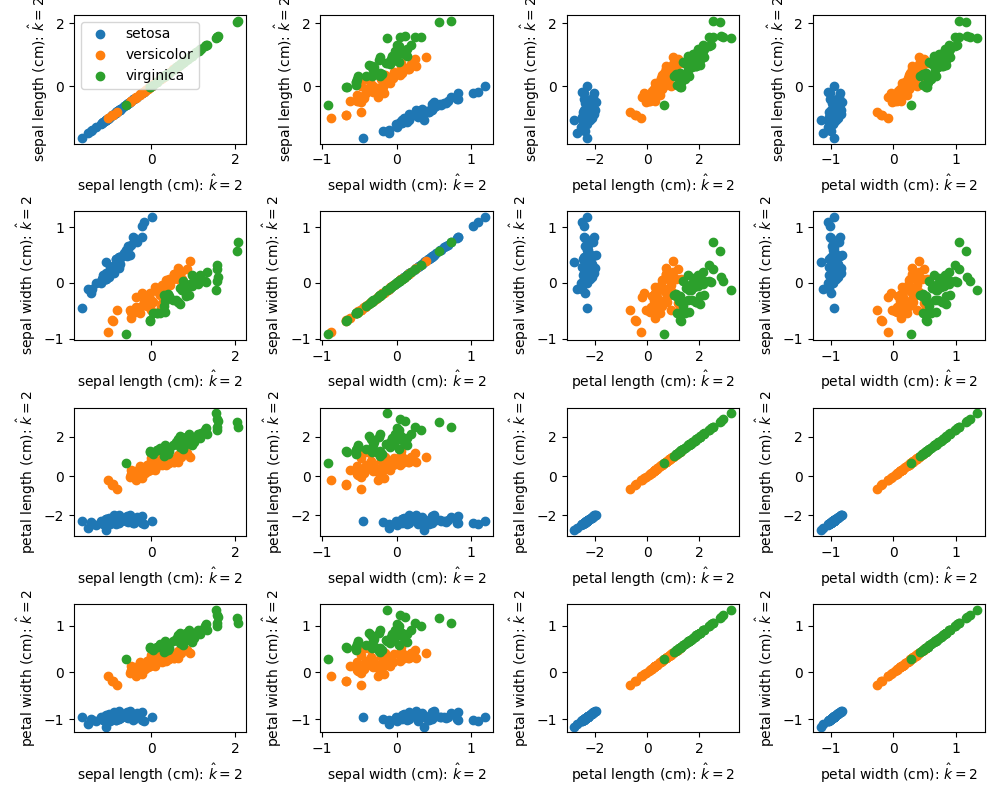
\includegraphics[width=0.75\textwidth,height=\textheight]{bilder/05-all-pairs-k2-rec.png}
\caption{Pinguin Datenset -- rekonstruiert von \(\hat k =2\) Hauptachsenkoordinaten}\label{fig:05-penguin-allpairs-k2-rec}
}
\end{figure}

\hypertarget{aufgaben-2}{%
\section{Aufgaben}\label{aufgaben-2}}

\hypertarget{kovarianzen-pt}{%
\subsection{Kovarianzen (P+T)}\label{kovarianzen-pt}}

Erzeugen Sie für \texttt{N} aus \texttt{Nl\ =\ {[}10,\ 1000,\ 100000{]}} zufällige Vektoren \texttt{x} und \texttt{y} der Länge \texttt{N} und berechnen Sie
für den Datensatz \texttt{X\ =\ {[}x,\ x,\ x*y,\ y{]}}
jeweils die Matrix der Korrelationskoeffizienten
\begin{equation*}
\rho _{i\;j} = \frac{s_{i\, j}}{s_i \cdot s_j}
\end{equation*}
wobei \(s_{i\,j}\) die Kovarianz der Daten \({\mathbf{x} _ i}\) und \({\mathbf{x} _ j}\) ist und \(s_{i}\) die Varianz von \({\mathbf{x} _ i}\). Interpretieren sie die Ergebnisse.

\textbf{Hinweis}: Weil Zufälligkeit involviert ist, ist die Interpretation manchmal schwierig. Lassen sie das Programm öfter laufen und beobachten sie verschiedene Realisierungen der Stichproben.

\begin{Shaded}
\begin{Highlighting}[]
\ImportTok{import}\NormalTok{ numpy }\ImportTok{as}\NormalTok{ np}

\CommentTok{# N = 10}

\NormalTok{x }\OperatorTok{=}\NormalTok{ np.random.randn(}\DecValTok{10}\NormalTok{, }\DecValTok{1}\NormalTok{)}
\NormalTok{y }\OperatorTok{=}\NormalTok{ np.random.randn(}\DecValTok{10}\NormalTok{, }\DecValTok{1}\NormalTok{)}

\NormalTok{X }\OperatorTok{=}\NormalTok{ np.hstack([x, x, x}\OperatorTok{*}\NormalTok{y, y])}

\NormalTok{Xcntrd }\OperatorTok{=}\NormalTok{ X }\OperatorTok{-}\NormalTok{ X.mean(axis}\OperatorTok{=}\DecValTok{0}\NormalTok{)}
\CommentTok{# zentrieren der Daten}

\CommentTok{# Kovarianz Matrix ausrechnen}
\NormalTok{covX }\OperatorTok{=} \DecValTok{1}\OperatorTok{/}\NormalTok{(}\DecValTok{10-1}\NormalTok{)}\OperatorTok{*}\NormalTok{Xcntrd.T }\OperatorTok{@}\NormalTok{ Xcntrd}

\CommentTok{# Varianzen -- stehen auf der Diagonalen im Quadrat}
\NormalTok{varvec }\OperatorTok{=}\NormalTok{ np.sqrt(np.diagonal(covX)).reshape(}\DecValTok{4}\NormalTok{, }\DecValTok{1}\NormalTok{)}
\CommentTok{# Matrix mit den Kombinationen aller Varianzen}
\NormalTok{varmat }\OperatorTok{=}\NormalTok{ varvec }\OperatorTok{@}\NormalTok{ varvec.T}

\NormalTok{matcc }\OperatorTok{=}\NormalTok{ covX }\OperatorTok{*} \DecValTok{1}\OperatorTok{/}\NormalTok{varmat}

\BuiltInTok{print}\NormalTok{(}\SpecialStringTok{f'N=}\SpecialCharTok{\{}\DecValTok{10}\SpecialCharTok{\}}\SpecialStringTok{ : Matrix of Correlation Coefficients='}\NormalTok{)}
\BuiltInTok{print}\NormalTok{(matcc)}
\end{Highlighting}
\end{Shaded}

\hypertarget{pinguin-datensatz-targets-plotten-p}{%
\subsection{Pinguin Datensatz -- Targets Plotten (P)}\label{pinguin-datensatz-targets-plotten-p}}

Laden Sie die \href{bilder/penguin-data.json}{Pinguin Datensatz} (hier als \texttt{json} file bereitgestellt) und plotten sie \texttt{petal\ width} versus \texttt{sepal\ length} für die drei Spezies \texttt{setosa}, \texttt{versicolor}, \texttt{virginica} in drei separaten Grafiken.

\begin{Shaded}
\begin{Highlighting}[]
\ImportTok{import}\NormalTok{ json}

\ImportTok{import}\NormalTok{ numpy }\ImportTok{as}\NormalTok{ np}
\ImportTok{import}\NormalTok{ matplotlib.pyplot }\ImportTok{as}\NormalTok{ plt}

\ControlFlowTok{with} \BuiltInTok{open}\NormalTok{(}\StringTok{'penguin-data.json'}\NormalTok{, }\StringTok{'r'}\NormalTok{) }\ImportTok{as}\NormalTok{ f:}
\NormalTok{    datadict }\OperatorTok{=}\NormalTok{ json.load(f)}

\BuiltInTok{print}\NormalTok{(datadict.keys())}

\NormalTok{data }\OperatorTok{=}\NormalTok{ np.array(datadict[}\StringTok{'data'}\NormalTok{])}
\NormalTok{target }\OperatorTok{=}\NormalTok{ np.array(datadict[}\StringTok{'target'}\NormalTok{])}
\NormalTok{feature_names }\OperatorTok{=}\NormalTok{ datadict[}\StringTok{'feature_names'}\NormalTok{]}
\NormalTok{target_names }\OperatorTok{=}\NormalTok{ datadict[}\StringTok{'target_names'}\NormalTok{]}

\BuiltInTok{print}\NormalTok{(}\StringTok{'target names: '}\NormalTok{, target_names)}
\BuiltInTok{print}\NormalTok{(}\StringTok{'feature names: '}\NormalTok{, feature_names)}

\NormalTok{fig, axs }\OperatorTok{=}\NormalTok{ plt.subplots(nrows}\OperatorTok{=}\DecValTok{1}\NormalTok{, ncols}\OperatorTok{=}\DecValTok{3}\NormalTok{, figsize}\OperatorTok{=}\NormalTok{(}\DecValTok{10}\NormalTok{, }\DecValTok{3}\NormalTok{))}

\CommentTok{# # Ein Vektor der aus dem Target Vektor das target 0 raussucht}
\NormalTok{trgtidx_z }\OperatorTok{=}\NormalTok{ (target }\OperatorTok{==} \DecValTok{0}\NormalTok{)}
\CommentTok{# # Wird gleich benutzt um die Daten nach diesem target zu filtern}

\NormalTok{target_z_daten }\OperatorTok{=}\NormalTok{ data[trgtidx_z, :]}

\NormalTok{axs[}\DecValTok{0}\NormalTok{].plot(target_z_daten[:, }\DecValTok{3}\NormalTok{], target_z_daten[:, }\DecValTok{0}\NormalTok{],}
            \StringTok{'o'}\NormalTok{, label}\OperatorTok{=}\NormalTok{target_names[}\DecValTok{0}\NormalTok{])}

\NormalTok{axs[}\DecValTok{0}\NormalTok{].legend()}
\NormalTok{axs[}\DecValTok{0}\NormalTok{].set_xlabel(feature_names[}\DecValTok{3}\NormalTok{])}
\NormalTok{axs[}\DecValTok{0}\NormalTok{].set_ylabel(feature_names[}\DecValTok{0}\NormalTok{])}
\NormalTok{axs[}\DecValTok{0}\NormalTok{].set_title(target_names[}\DecValTok{0}\NormalTok{])}

\NormalTok{plt.tight_layout()}
\NormalTok{plt.show()}
\end{Highlighting}
\end{Shaded}

Hier wurden die \texttt{python} Datentypen

\begin{itemize}
\tightlist
\item
  \emph{list} -- z.B. \texttt{datenpunkte\ =\ {[}1,\ 2,\ 3{]}}
\item
  \emph{array} -- z.B. \texttt{datenmatrix\ =\ np.array(datenpunkte)}
\item
  \emph{dictionary} -- z.B. \texttt{datadict\ =\ \{\textquotesingle{}data\textquotesingle{}:\ datenpunkte\}}
\end{itemize}

verwendet, die alle für verschiedene Zwecke gerne benutzt werden. Z.B.

\begin{itemize}
\tightlist
\item
  Liste -- als eine Sammlung von (möglicherweise total unterschiedlichen) Objekten, über die iteriert werden kann und die einfach zu erweitern ist
\item
  \texttt{arrays} -- Matrix/Vektor von Daten eines Typs, mit denen \emph{gerechnet} werden kann
\item
  \texttt{dictionaries} -- ein \emph{Lookup table}. Objekte können über einen Namen addressiert werden. Ich nehme sie gerne um Daten mit ihrem Namen zum Beispiel als \texttt{json} file zu speichern.
\end{itemize}

\hypertarget{pinguin-datensatz-2d-plots-p}{%
\subsection{Pinguin Datensatz -- 2D plots (P)}\label{pinguin-datensatz-2d-plots-p}}

Erzeugen sie Abbildung \ref{fig:05-penguin-allpairs} zum Beispiel über ein \texttt{4x4} Feld von subplots

\begin{Shaded}
\begin{Highlighting}[]
\NormalTok{fig, axs }\OperatorTok{=}\NormalTok{ plt.subplots(nrows}\OperatorTok{=}\DecValTok{4}\NormalTok{, ncols}\OperatorTok{=}\DecValTok{4}\NormalTok{, figsize}\OperatorTok{=}\NormalTok{(}\DecValTok{10}\NormalTok{, }\DecValTok{8}\NormalTok{))}
\end{Highlighting}
\end{Shaded}

erzeugen, in das sie mittels

\begin{Shaded}
\begin{Highlighting}[]
\NormalTok{axs[zeile, spalte].plot(xdaten, ydaten, }\StringTok{'o'}\NormalTok{)}
\end{Highlighting}
\end{Shaded}

die plots fuer die einzelnen targets ``eintragen'' koennen. Bitte die Achsen beschriften (die \texttt{legend} ist nicht unbedingt notwendig).

\hypertarget{kovarianz-p}{%
\subsection{Kovarianz (P)}\label{kovarianz-p}}

Zentrieren Sie den Datensatz (zum Beispiel unter Verwendung der \texttt{numpy.mean} Funktion) und berechnen Sie die Kovarianzmatrix.

\hypertarget{hauptachsentransformation-p}{%
\subsection{Hauptachsentransformation (P)}\label{hauptachsentransformation-p}}

Berechnen sie Hauptachsen und stellen Sie die Daten in den Hauptachsenkoordinaten dar (wie in Abbildung \ref{fig:05-penguin-allpairs-pcs}).

\hypertarget{kovarianzmatrix-t}{%
\subsection{Kovarianzmatrix (T)}\label{kovarianzmatrix-t}}

Zeigen sie, dass für zentrierte Datensätze \({\mathbf{X}}\in \mathbb R^{N\times n}\) gilt, dass
\begin{equation*}
\operatorname{Cov}(X) = \frac{1}{N-1}{\mathbf{X}}^T{\mathbf{X}}.
\end{equation*}

\hypertarget{gesamtvarianz-t}{%
\subsection{Gesamtvarianz (T)}\label{gesamtvarianz-t}}

Zeigen sie, dass auch für \(n>2\) die Summe der Varianzen in orthogonalen Achsenrichtungen unabhängig von der Wahl des Koordinatensystems sind. (Vergleiche Kapitel 4.2 Koordinatenwechsel)

\end{document}
